%!TEX TS-program = pdflatex
%!TEX encoding = utf8
\documentclass[12pt, twoside]{book} 
\usepackage[T1]{fontenc}
\usepackage[utf8]{inputenc}
\usepackage[english, spanish, es-noshorthands]{babel}
%% FONTS: libertine+biolinum+stix
\usepackage[mono=false]{libertine}
\usepackage[notext]{stix}
\usepackage{float}
\usepackage{epsfig}
\usepackage{listings}

% =====================
% = Datos importantes =
% =====================
% hay que rellenar estos datos y luego
% ir a \begin{document}

\title{Desarrollo de proyectos IoT utilizando Raspberry Pi como plataforma}
\author{Miguel Ángel Martínez Sánchez}
\date{\today}
\newcommand{\tutores}[1]{\newcommand{\guardatutores}{#1}}
\tutores{Prof. Tutor Primero Apellido Apellido\\
         Prof. Tutor Segundo Apellido Apellido\\
         Prof. Tutor Tercero Apellido Apellido}

% ======================
% = Páginas de títulos =
% ======================
\makeatletter
\edef\maintitle{\@title}
\renewcommand\maketitle{%
  \begin{titlepage}
      \vspace*{1.5cm}
      \parskip=0pt
      \Huge\bfseries
      \begin{center}
          \leavevmode
\includegraphics[totalheight=6cm]{sello.png}\\[2cm]
          \@title
      \end{center}
      \vspace{1cm}
      \begin{center}
          \@author
      \end{center}
  \end{titlepage}
  
  \begin{titlepage}
  \parindent=0pt
  \begin{flushleft}
  \vspace*{1.5mm}
  \setlength\baselineskip{0pt}
  \setlength\parskip{0mm}
  \begin{center}
      \leavevmode
\includegraphics[totalheight=4.5cm]{sello.png}
  \end{center}
  \end{flushleft}
  \vspace{1cm}
  \bgroup
  \Large \bfseries
  \begin{center}
  \@title
  \end{center}
  \egroup
  \vspace*{.5cm}
  \begin{center}
  \@author
  \end{center}
  \vspace*{1.8cm}
  \begin{flushright}
  \begin{minipage}{8.45cm}

      \vspace*{7.5mm}

      Tutorizada por
      % \vspace*{5mm}
  \end{minipage}\par
  \begin{tabularx}{8.45cm}[b]{@{}l}
      \guardatutores
  \end{tabularx}
   \end{flushright}
      \vspace*{\fill}
   \end{titlepage}
   %%% Esto es necesario...
   \pagestyle{tfg}
   \renewcommand{\chaptermark}[1]{\markright{\thechapter.\space ##1}}
   \renewcommand{\sectionmark}[1]{}
   \renewcommand{\subsectionmark}[1]{}
  }
\makeatother

% ======================================
% = Color de la Universidad de Sevilla =
% ======================================
\usepackage{tikz}
\definecolor{USred}{cmyk}{0,1.00,0.65,0.34}

% =========
% = Otros =
% =========
\usepackage[]{tabularx}
\usepackage[]{enumitem}
\setlist{noitemsep}

% ==========================
% = Matemáticas y teoremas =
% ==========================
\usepackage[]{amsmath}
\usepackage[]{amsthm}
\usepackage[]{mathtools}
\usepackage[]{bm}
\usepackage[]{thmtools}
\newcommand{\marcador}{\vrule height 10pt depth 2pt width 2pt \hskip .5em\relax}
\newcommand{\cabeceraespecial}{%
    \color{USred}%
    \normalfont\bfseries}
\declaretheoremstyle[
    spaceabove=\medskipamount,
    spacebelow=\medskipamount,
    headfont=\cabeceraespecial\marcador,
    notefont=\cabeceraespecial,
    notebraces={(}{)},
    bodyfont=\normalfont\itshape,
    postheadspace=1em,
    numberwithin=chapter,
    headindent=0pt,
    headpunct={.}
    ]{importante}
\declaretheoremstyle[
    spaceabove=\medskipamount,
    spacebelow=\medskipamount,
    headfont=\normalfont\itshape\color{USred},
    notefont=\normalfont,
    notebraces={(}{)},
    bodyfont=\normalfont,
    postheadspace=1em,
    numberwithin=chapter,
    headindent=0pt,
    headpunct={.}
    ]{normal}
\declaretheoremstyle[
    spaceabove=\medskipamount,
    spacebelow=\medskipamount,
    headfont=\normalfont\itshape\color{USred},
    notefont=\normalfont,
    notebraces={(}{)},
    bodyfont=\normalfont,
    postheadspace=1em,
    headindent=0pt,
    headpunct={.},
    numbered=no,
    qed=\color{USred}\marcador
    ]{demostracion}

% Los nombres de los enunciados. Añade los que necesites.
\declaretheorem[name=Observaci\'on, style=normal]{remark}
\declaretheorem[name=Corolario, style=normal]{corollary}
\declaretheorem[name=Proposici\'on, style=normal]{proposition}
\declaretheorem[name=Lema, style=normal]{lemma}

\declaretheorem[name=Teorema, style=importante]{theorem}
\declaretheorem[name=Definici\'on, style=importante]{definition}

\let\proof=\undefined
\declaretheorem[name=Demostraci\'on, style=demostracion]{proof}


% ============================
% = Composición de la página =
% ============================
\usepackage[
	a4paper,
    textwidth=80ex,
]{geometry}

\linespread{1.069}
\parskip=10pt plus 1pt minus .5pt
\frenchspacing
% \raggedright


% ==============================
% = Composición de los títulos =
% ==============================

\usepackage[explicit]{titlesec}

\newcommand{\hsp}{\hspace{20pt}}
\titleformat{\chapter}[hang]
    {\Huge\sffamily\bfseries}
    {\thechapter\hsp\textcolor{USred}{\vrule width 2pt}\hsp}{0pt}
    {#1}
\titleformat{\section}
  {\normalfont\Large\sffamily\bfseries}{\thesection\space\space}
  {1ex}
  {#1}
\titleformat{\subsection}
  {\normalfont\large\sffamily}{\thesubsection\space\space}
  {1ex}
  {#1}

% =======================
% = Cabeceras de página =
% =======================
\usepackage[]{fancyhdr}
\usepackage[]{emptypage}
\fancypagestyle{plain}{%
    \fancyhf{}%
    \renewcommand{\headrulewidth}{0pt}
    \renewcommand{\footrulewidth}{0pt}
}
\fancypagestyle{tfg}{%
    \fancyhf{}%
    \renewcommand{\headrulewidth}{0pt}
    \renewcommand{\footrulewidth}{0pt}
    \fancyhead[LE]{{\normalsize\color{USred}\bfseries\thepage}\quad
                    \small\textsc{\MakeLowercase{\maintitle}}}
    \fancyhead[RO]{\small\textsc{\MakeLowercase{\rightmark}}%
                    \quad{\normalsize\bfseries\color{USred}\thepage}}%
                    }

\usepackage{xcolor}
\usepackage[colorlinks = true,
            linkcolor = blue,
            urlcolor  = blue,
            citecolor = blue,
            anchorcolor = blue]{hyperref}
\newcommand{\MYhref}[3][blue]{\href{#2}{\color{#1}{#3}}}
% =============================
% = El documento empieza aquí =
% =============================
\begin{document}
 

\maketitle

\frontmatter
\tableofcontents

\mainmatter


\chapter*{English Abstract}
\addcontentsline{toc}{chapter}{English Abstract}
\markright{English Abstract}



\begin{otherlanguage}{english}
    According to the guidelines, every dissertation should include a short english abstract at the beginning. In the abstract, you describe in general terms what is your dissertation about, the main points you want to make, and any important consequences that may arise.
\end{otherlanguage}

\chapter*{Agradecimientos}
\chapter{Los enunciados}

\section{Teoremas y demostraciones}


\begin{theorem}[Euclides]\label{thm:th1}
    Esto es un Teorema. Se numeran a partir del 1 en cada capítulo. Como son importantes, tienen un cuadrado rojo al principio. Llevan letra cursiva.
\end{theorem}

\begin{proof}
    Esto es la demostración. Al final de la demostración se puede ver un cuadrado rojo similar al de los teoremas. Las demostraciones no llevan letra cursiva.
\end{proof}


\begin{definition}\label{def:1}
    Esto es una definición. Las definiciones son importantes; también llevan un cuadradito rojo.
\end{definition}


\subsection{Otros enunciados}


\begin{remark}
    Esto es una observación, que dice que $e=mc^{2}$. Como las observaciones no son importantes, no llevan cuadrado rojo, y el tipo de letra no es cursiva.
\end{remark}


\begin{proof}
    Si la demostración acaba en una fórmula, para poner el cuadrado rojo a la altura de la última formula, hay que usar la orden \verb|\qedhere|, como en este caso:
    \[
        e=mc^{2}.\qedhere
    \]

\end{proof}


\begin{corollary}\label{cor:1}
    Esto es un corolario.
\end{corollary}

\begin{proposition}\label{pro:1}
    Esto es una proposición.
\end{proposition}

\begin{lemma}[Gauss]\label{lem:1}
    Esto es un lema.
\end{lemma}


\backmatter

\bibliographystyle{acm}
% \biliography{miarchivo} % -> lee miarchivo.bib


\chapter{MQTT}

\section{MQTT}
MQTT(Message Queue Telemetry Transport) es un protocolo usado para la comunicación M2M (Machine to machine) en el internet de las cosas. Fue creado por IBM en 1999. Está orientado a las redes de dispositivos pequeños, como sensores, debido a que consume muy poco ancho de banda. Se ha convertido en un protocolo muy usado en IoT, aunque también es ideal para aplicaciones móviles por su envío eficiente. Un ejemplo de uso es Facebook Messenger para iPhone y Android.\\
Se basa en el estandar publish/subscribe usado sobre TCP/IP. Esta comunicación publish/subscribe necesita de un "broker" o servidor para transmitir los paquetes.

\begin{figure}[h!]
\centering
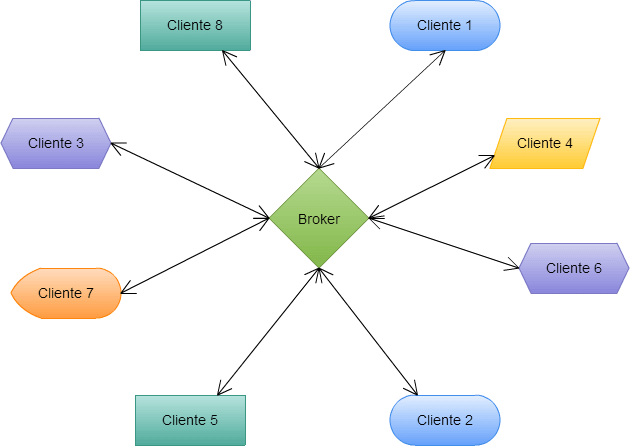
\includegraphics[scale=0.3]{images/topologia.png}
\caption{Topología MQTT.}\label{L401}
\end{figure}
\newpage
%\vspace*{1.8cm}
La comunicación se basa en "topics" (temas) que el cliente que publica el mensaje envía y los nodos que desean recibirlo deben subscribirse a él. Un topic se representa mediante una cadena de caracteres separada por "/". De esta forma se pueden crear jerarquías como se puede ver en la figura \ref{L402} \\ 
\begin{figure}[h!]
\centering
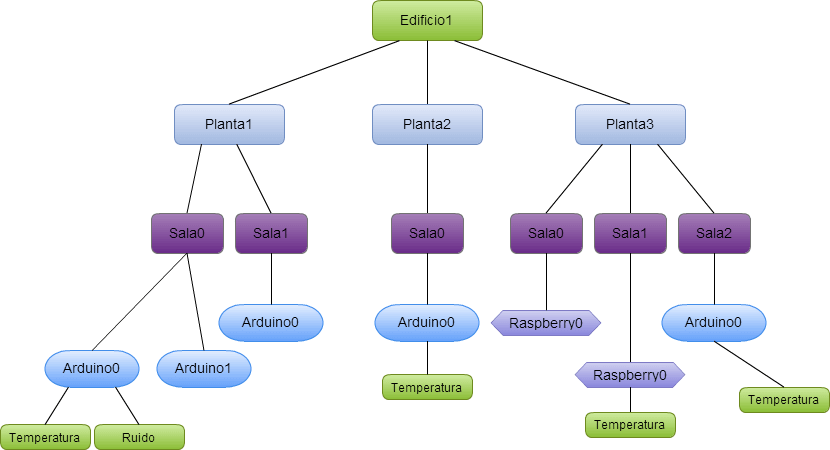
\includegraphics[scale=0.3]{images/jerarquia.png}
\caption{Jerarquía Topics.}\label{L402}
\end{figure}

\section{Requisitos}
MQTT como middleware IoT, necesita cumplir una serie de requisitos. En el escenario que se plantea hay algunos que no son indispensables y otro que sí lo son, como pueda ser la seguridad. Aquí se definen algunos de los requisitos.
\subsection{Escalabilidad}
MQTT tiene, en general, una alta escalabilidad, que va a depender en gran medida de la calidad de los nodos y de la topología que se use. La existencia de uno o más brokers dota al sistema de gran escalabilidad ya que la solución puede crecer solo con aumentar recursos en un único elemento.
Para añadir un nuevo cliente, tan solo es necesario suscribirse a un topic.
\begin{figure}[h!]
\centering
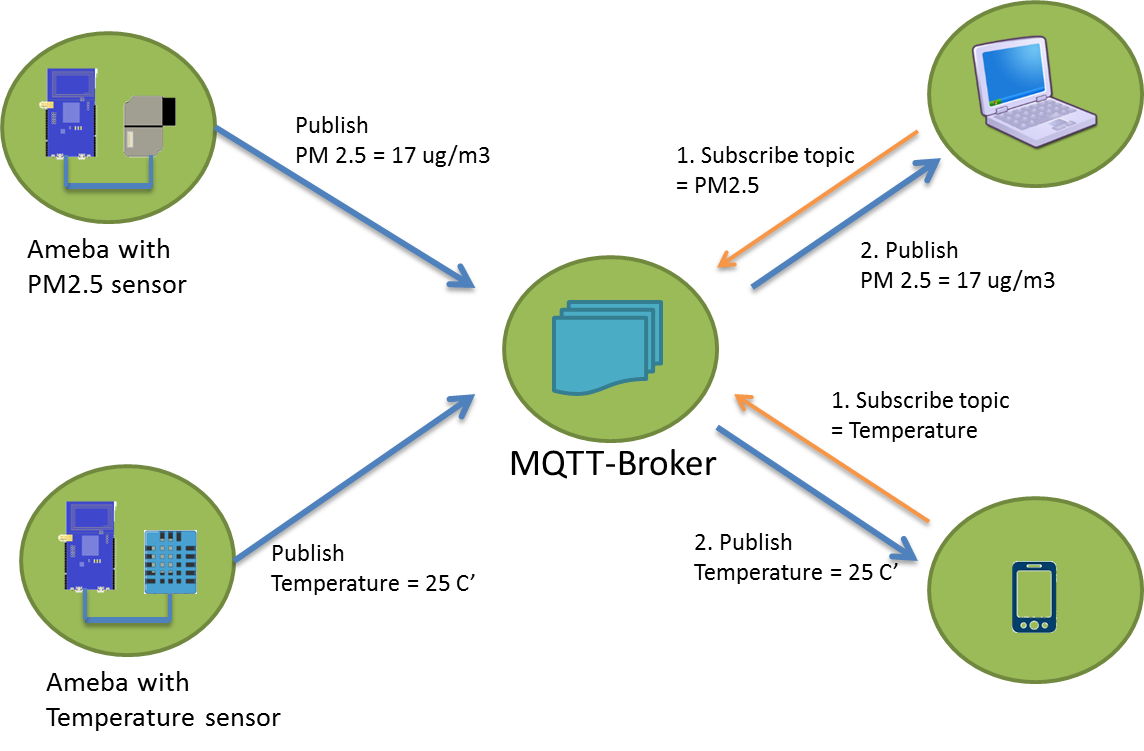
\includegraphics[scale=0.3]{images/figure3.png}
\caption{Escalabilidad MQTT}\label{L403}
\end{figure}
\subsection{Seguridad}
La seguridad es vital en un entorno IoT y para ello MQTT usa TLS junto con una autenticación de usuario/contraseña. Usa una autenticación usuario/contraseña a nivel de aplicación para establecer la conexión entre cliente y broker. Si TLS se resuelve correctamente, entra en juego dicha autenticación. Además, también existen políticas de autorización para denegar un determinado topic o para permitir una operación
\begin{figure}[h!]
\centering
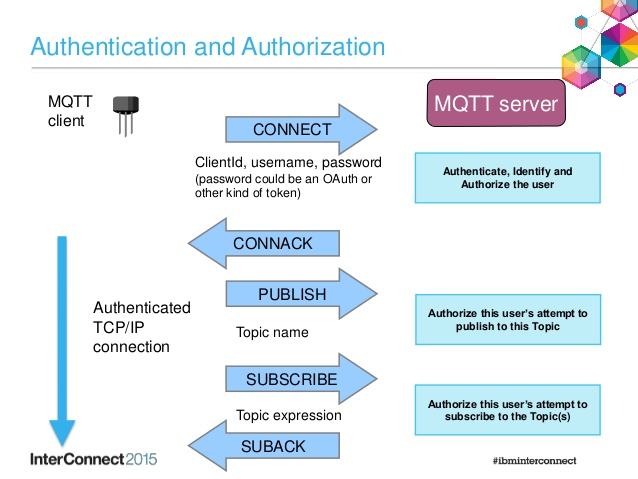
\includegraphics[scale=0.3]{images/mqtt_ssl}
\caption{Autenticación MQTT}\label{L404}
\end{figure}
\subsection{Disponibilidad}
MQTT no tiene una gran disponibilidad, aunque con herramientas como balanceadores de carga, o el uso de los brokers en modo “bridge” se puede conseguir una buena disponibilidad. La disponibilidad permitirá poder seguir usando la red en caso de fallo en alguno de sus nodos.
\begin{figure}[h!]
\centering
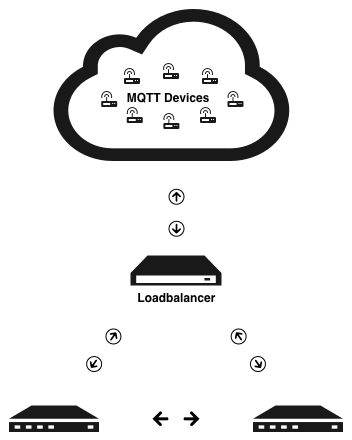
\includegraphics[scale=0.3]{images/mqtt_availability.png}
\caption{Balanceador de carga en MQTT}\label{L405}
\end{figure}
\subsection{Confiabilidad}
MQTT proporciona 3 grados de QoS para la entrega de los paquetes:
\begin{itemize}
\item[•]\textbf{QoS 0: Como mucho una vez}\\
El mensaje PUBLISH se envía y el broker no manda ningún reconocimiento. El mensaje llega al broker una vez o ninguna y si llega, llegará a los subscriptores una vez o ninguna.
\begin{figure}[h!]
\centering
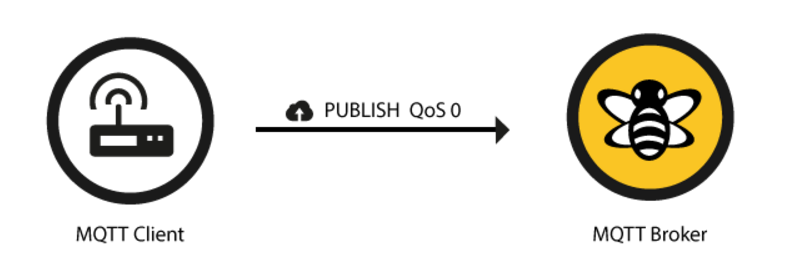
\includegraphics[scale=0.3]{images/qos0}
\caption{QoS 0}\label{L406}
\end{figure}
\item[•]\textbf{QoS 1: Al menos una vez}\\
Este nivel de calidad de servicio asegura que llega al broker al menos una vez. El broker tiene que reconocer la recepción con un paquete PUBACK. Si no recibe un acuse de recibo se vuelve a enviar de nuevo el mensaje PUBLISH con otro identificador distinto hasta que se reciba el reconocimiento. En este nivel no se garantiza que los paquetes no lleguen duplicados.
\begin{figure}[H]
\centering
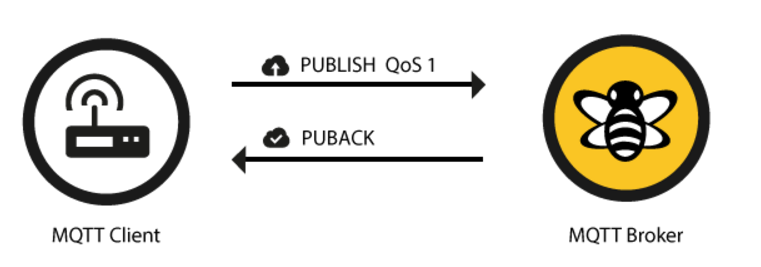
\includegraphics[scale=0.3]{images/qos1}
\caption{QoS 1}\label{L407}
\end{figure}
\item[•] \textbf{QoS 2: Exactamente una vez}\\
Este nivel de calidad asegura que el paquete llega una y solo una vez. Para ello se deben enviar además los paquetes PUBREC y PUBREL.
\begin{figure}[h!]
\centering
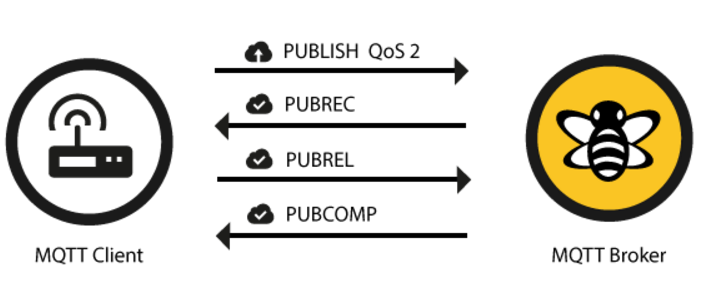
\includegraphics[scale=0.3]{images/qos2}
\caption{QoS 2}\label{L408}
\end{figure}
\end{itemize}
\subsection{Tiempo real}
Si tiempo real lo definimos en microsegundos, MQTT no cumple este requisito ya que una de las principales características de MQTT es que funciona sobre TCP. En el escenario que se plantea, estos microsegundos no son necesarios por lo que no es un requisito indispensable.
\subsection{Control de datos}
MQTT proporciona un control de datos como son el almacenamiento o el filtrado. De todo ello se encarga el broker. El broker puede almacenar los paquetes de un tópico mientras el cliente, subscrito a dicho tópico, esté offline. El broker también puede aplicar un filtrado en los tópicos, para que se aplique a un nivel o a todos los niveles de ese tópico:
\begin{itemize}
\item[•]\textbf{Single level : +} \\
\begin{figure}[h!]
\centering
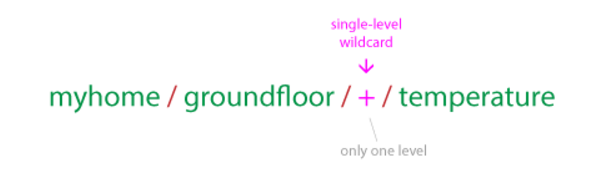
\includegraphics[scale=0.5]{images/figure4}
\caption{Single level}\label{L409}
\end{figure}
Para que el mensaje llegue a un cliente, éste debe de estar subscrito a un tópico en el que solamente cambie el nivel indicado por el signo +. En este ejemplo, el mensaje destinado a \textbf{myhome/groundfloor/livingroom/temperature} o \textbf{myhome/groundfloor/kitchen/temperature} llegaría al cliente. Sin embargo, un mensaje destinado a \textbf{myhome/groundfloor/kitchen/brightness} o \textbf{myhome/firstfloor/kitchen/temperature} no llegaría al cliente.
\item[•]\textbf{Multi level: \#}\\
\begin{figure}[h!]
\centering
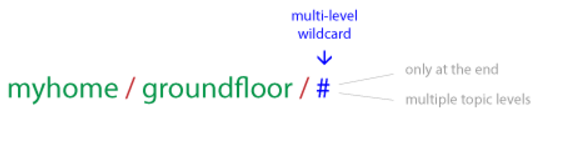
\includegraphics[scale=0.5]{images/figure5}
\caption{Multi level}\label{L410}
\end{figure}
En este caso, llegaría a cualquier cliente que esté subscrito a partir de ese nivel.\\
Los tópicos que empiecen por el símbolo \$ están reservados para las estadísticas internas del broker MQTT. Un ejemplo puede ser:
\begin{itemize}
\item[•]\$SYS/broker/clients/connected
\item[•]\$SYS/broker/clients/disconnected
\item[•]\$SYS/broker/clients/total
\item[•]\$SYS/broker/messages/sent
\end{itemize}
\end{itemize}
\subsection{Descubrimiento de recursos}
En MQTT no hay un mecanismo para el descubrimiento de recursos. El cliente se tiene que conectar al broker para su comunicación. Con MQTT-SN, una extensión de MQTT para redes de sensores, sí que hay un mecanismo de descubrimiento de nuevos dispositivos.
\subsection{Documentación e interoperabilidad}
MQTT es un middleware de código abierto perfectamente documentado en\\
%\MYhref{ http://docs.oasis-open.org/mqtt/mqtt/v3.1.1/mqtt-v3.1.1.html}{Google}
\url{ http://docs.oasis-open.org/mqtt/mqtt/v3.1.1/mqtt-v3.1.1.html}

MQTT es un protocolo heterogéneo en cuanto a dispositivos y tecnologías se refiere. Puede funcionar prácticamente en cualquier dispositivo ya que es un protocolo muy sencillo que requiere poco procesamiento. Puede funcionar en un dispositivo móvil, PC, Raspberry… 





\chapter{MQTT-SN}
\section{Redes de sensores inalámbricas}
Las redes de sensores o Wireless Sensor Networks (WSN) en inglés, se han incrementado en los últimos años. Estas redes tienen diferentes aplicaciones, como puede ser la vigilancia y seguridadd, medicina, domótica o aplicaciones militares. Una red de sensores está formada por sensores y gateway para conectar con una red de datos. En estas redes es importante la comunicación de forma inalambrica entre sensores, puesto que el número de nodos (sensores, actuadores...) es muy grande, y una infraestructura cableada tendría un coste muy elevado. Las características de estas redes son:
\begin{itemize}
\item[•]Tolerancia a fallos\\
\item[•]Coste\\
\item[•]Ausencia de infraestructura de red\\
\item[•]Bajo consumo
\end{itemize} 
A diferencia de las redes convencionales, los nodos no tienen conocimiento de la topología de la red, por lo que el enrutamiento cambia con respecto a éstas. Aquí es el nodo es el que se informa de sus nuevos nodos a su alcance y de la manera de encaminarse hacia ellos. En la figura \ref{L411} se puede ver la estructura de una red de este tipo.
\begin{figure}[H]
\centering
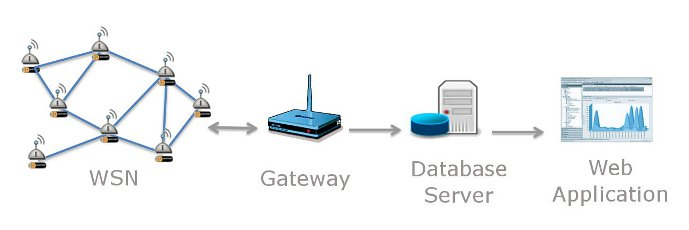
\includegraphics[scale=0.5]{images/wsn}
\caption{Multi level}\label{L411}
\end{figure}
 
\section{MQTT-SN}
MQTT es un protocolo usado sobre redes donde el ancho de banda sea limitado, sin embargo MQTT requiere del protocolo TCP/IP, útil para redes con dispositivos de aceptable procesamiento, puesto que ofrece una entrega correcta de los paquetes pero es demasiado complejo como para ser usado en redes de sensores, en las que los dispositivos son de poca memoria y de bajo procesamiento.\\
Es por ello donde surge MQTT-SN, un protocolo pub/sub específico para redes de sensores. 
\section{Arquitectura MQTT-SN}
La arquitectura MQTT-SN se muestra en la figura \ref{L412}
\begin{figure}[H]
\centering
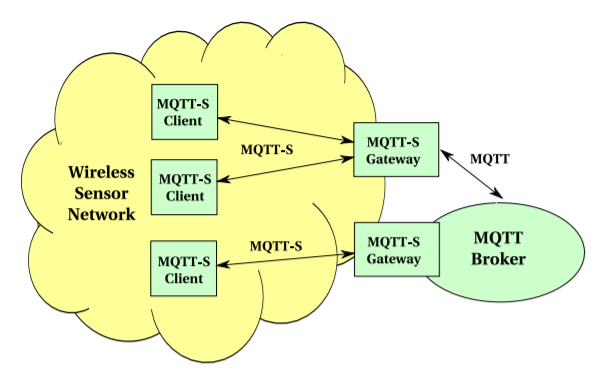
\includegraphics[scale=0.5]{images/mqttsn}
\caption{Arquitectura MQTT-SN}\label{L412}
\end{figure}
Hay 2 componentes: MQTT-SN clientes y MQTT-SN gateways. Los MQTT-SN clientes son los nodos en la red WSN. La comunicación entre clientes se hace a través del Gateway mediante el protocolo MQTT-SN. Los clientes realizan la comunicación pub/sub con un broker, localizado en una red tradicional, a través del Gateway. La comunicación entre el broker y el MQTT-Gateway se hace mediante el protocolo MQTT.
\section{Funcionamiento}  

\section{MQTT y MQTT-SN}


\chapter{OpenIoT}

\section{Introducción}
Aunque existen muchas aplicaciones IoT, cada una hace uso de servicios diferentes debido a que no hay un modelo a seguir para integrar todos los servicios.\\
En IoT no existe un estándar en cuanto a servicios se refiere, como sí existe en redes IP. OpenIoT surge como un proyecto europeo que busca la unificación de esas soluciones. \\
OpenIoT es una plataforma de código abierto que proporciona una interoperabilidad entre los servicios IoT en la nube. 
OpenIoT ofrece una infraestructura versátil para coleccionar datos de cualquier sensor disponible. Se hace uso también del concepto "datos enlazados", Linked Data en inglés. En el que los datos de los sensores se vinculan entre sí, para que puedan ser compartidos y entenderse entre ellos, ampliando así la información. Siempre buscando la principal característica en un entorno IoT, el Big Data. 

\section{Plataforma}
\subsection{Arquitectura}
La arquitectura de OpenIoT está formada en 7 elementos principales divididos en 3 planos lógicos, tal y como se puede observar en la figura \ref{L301}. 
\begin{figure}[H]
\centering
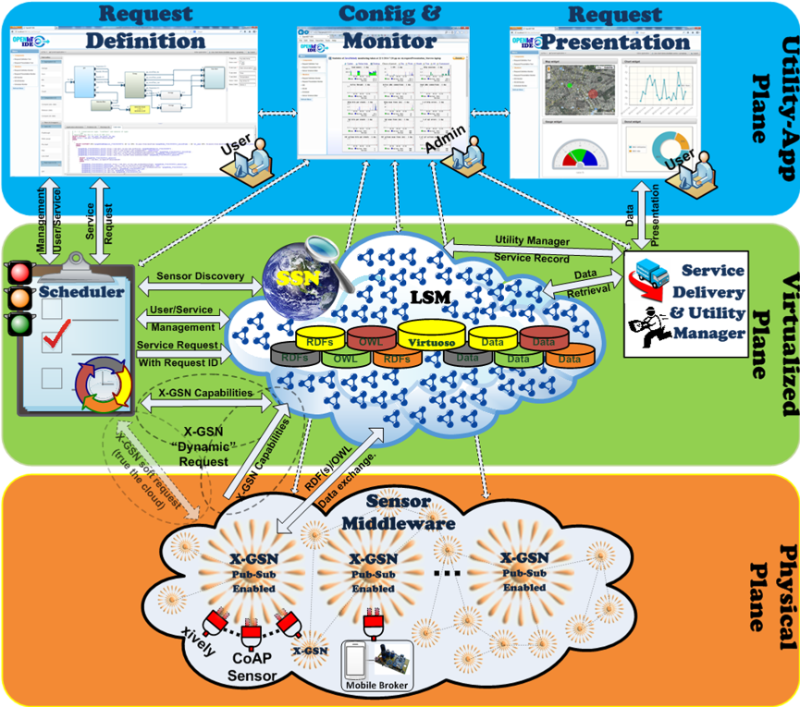
\includegraphics[scale=0.4]{images/openiot_platform1}
\caption{Arquitectura OpenIoT}\label{L301}
\end{figure}

El plano físico, virtualizado y un plano de utilidad. 
\begin{itemize}
\item[] \textbf{Plano físico}
\begin{itemize}
\item[•] \textbf{The sensor middleware}\\
Se encarga de filtrar, combinar y coleccionar los datos de los sensores. OpenIoT usa X-GSN como middleware, una versión extendida del middleware GSN. Además, se usa un middleware publish/subsribe para la integración de sensores móviles.
\end{itemize}
\end{itemize}
\begin{itemize}
\item[] \textbf{Plano virtual}
\begin{itemize}
\item[•] \textbf{The scheduler}\\
El scheduler o planificador procesa peticiones de los servicios y asegura su correcto acceso a los recursos que solicitan. Entre sus principales tareas está la de descubrir sensores.  \\
\item[•] \textbf{The cloud data storage}\\
Actúa como una base de datos en la nube, almacenando los datos enviados por los sensores. En OpenIoT se almacena también los metadatos asociados a esos datos.
OpenIoT usa Linked Stream Middleware Light (LSM-Light) \\
\item[•] \textbf{The Service Delivery \& Utility Manager} \\
Actúa, por un lado,combinando los flujos de datos para entregar el servicio solicitado. Hace uso de la descripción del servicio y de los recursos identificados por el Scheduler. Por otro lado, actúa como un servicio para realizar un seguimiento de las métricas de cada servicio (sensor). Como métricas se entiende la calidad, consumo, ancho de banda, volumen de datos...\\

\end{itemize}
\item[] \textbf{Plano de utilidad}
\begin{itemize}
\item[•] \textbf{The request definition} \\
Este componente proporciona una interfaz web para la especificación de las peticiones de un servicio.
\item[•] \textbf{The request presentation} \\
Se encarga de la visualización de los servicios de salida (mostrar gráficas,flujos de datos...)
\item[•] \textbf{The configuration and monitoring} \\
Se encarga del control y configuración de los sensores y servicios incluidos en la plataforma OpenIoT.
\end{itemize}
\end{itemize}
La figura \ref{L302} muestra la arquitectura de OpenIoT en bloques. Se pueden ver los diferentes servicios situados en cada plano. En el plano físico se muestra el middleware X-GSN y el middleware publish/subscribe para sensores móviles. Se muestra también, entre otros, el servicio de seguridad (CAS) o la plataforma de almacenamiento en la nube (LSM-Light), ambos pertenecientes al plano virtual. 

\begin{figure}[H]
\centering
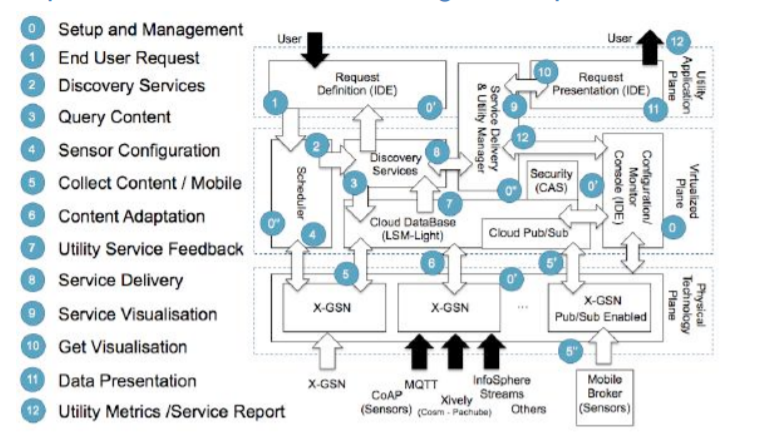
\includegraphics[scale=0.7]{images/blocks_openiot}
\caption{Bloques funcionales OpenIoT.}\label{L302}
\end{figure}

\subsubsection{Scheduler}
El Scheduler analiza cada petición de servicio y, de acuerdo con esto, interactúa con el resto de la plataforma OpenIoT, a través de la base de datos en la nube (Cloud DB). El scheduler tiene las siguientes funcionalidades:
\begin{itemize}
\item[•] \textbf{Descubridor de recursos}\\
Es capaz de descubrir los sensores virtuales disponibles a partir de la entidad "avaliableSensors" de su base de datos. Esta lista está basada en la sintaxis RDF cuando se envía a través de X-GSN.
\item[•] \textbf{Control de servicios}\\
El usuario puede llevar un control de los servicios. Para ello se usan comandos como "register", "suspend" , "unregister" o "update".
\item[•] \textbf{Actualizar recursos}\\
Un servicio que permite actualizar recursos
\item[•] \textbf{Obtener servicios}
Se usa para obtener la descripción de un determinado servicio ya registrado. 
\end{itemize}
Aunque el usuario pueda invocar a los distintos servicios, primero debe estar logueado correctamente dentro de la plataforma.
\subsubsection{Service delivery \& Utility Manager}
Las principales funciones de este servicio son:
\begin{itemize}
\item[•] Ejecutar y entregar los servicios pedidos.
\item[•] Procesar los flujos de datos de la nube.
\item[•] Seguimiento de los parámetros asociados al servicio. Por ejemplo, volumen de datos transmitidos o número de sensores usados.
\item[•] 
\end{itemize} 	
\subsection{Funcionalidades}

\subsubsection{Integración de datos enlazados}

Los datos enlazados es la forma que tiene la Web Semántica de vincular los distintos datos que están distribuidos en la web, así se puede llegar a la información relacionada que se hace referencia desde otros datos. Es decir, se le da una cierta capacidad de "razonar" a la web.
\begin{figure}[H]
\centering
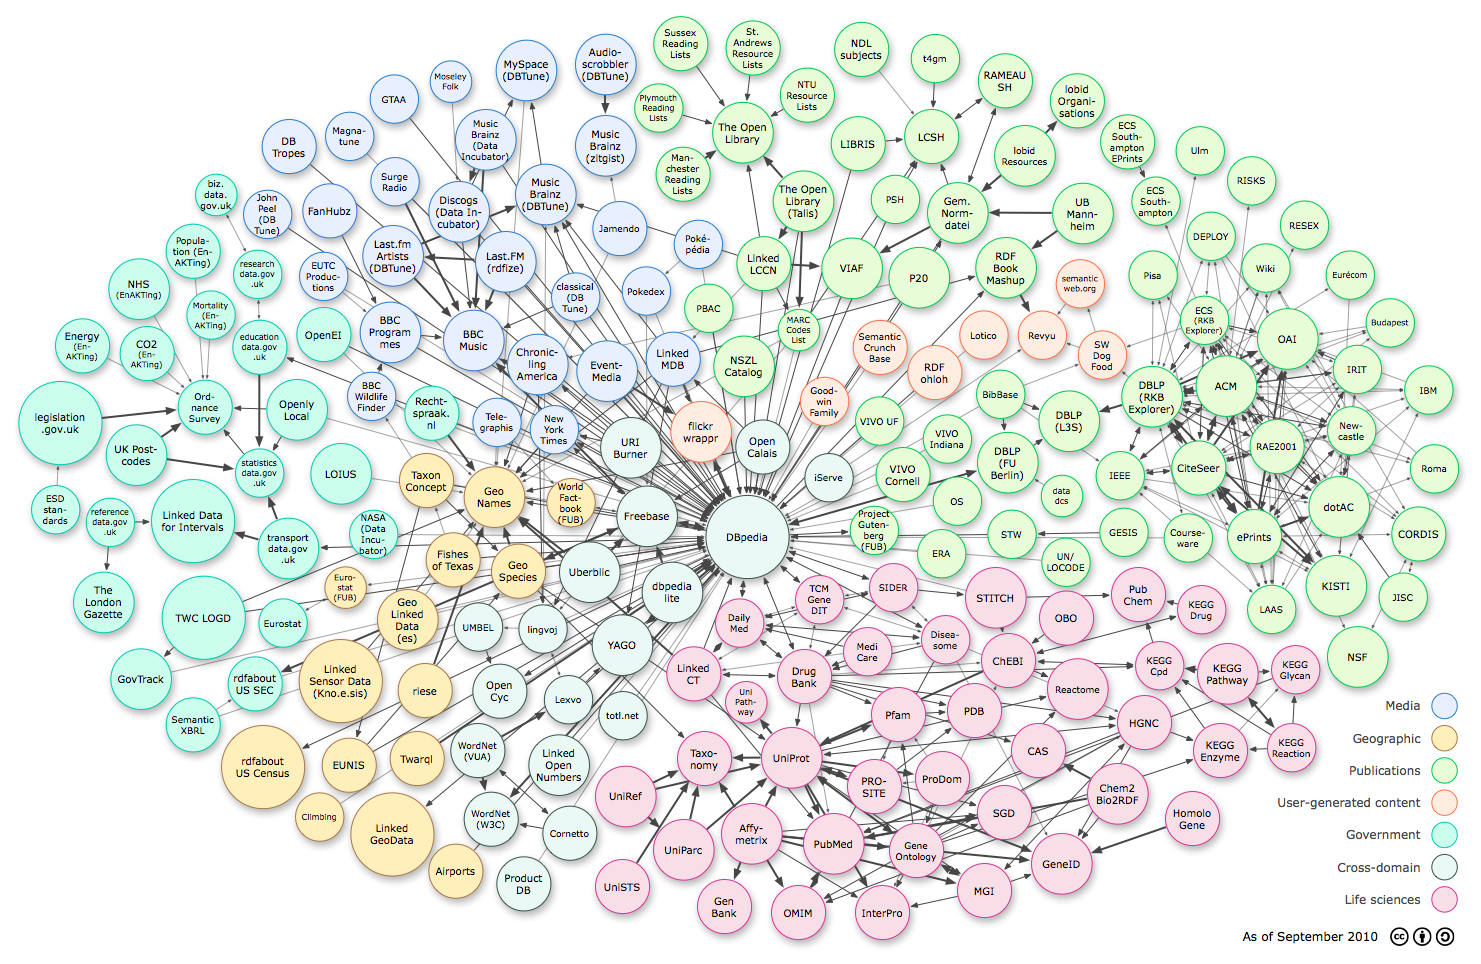
\includegraphics[scale=0.2]{images/linked_data}
\caption{Conjunto de datos vinculados entre sí en la web.}\label{L303}
\end{figure}

La principal funcionalidad de OpenIoT es el almacenamiento y procesado de datos, recopilados por sensores, en la nube. Y que estos datos puedan ser compartidos entre sí para poder ampliar la información. Es decir, hace uso del concepto de la web semántica. Para conseguir este concepto de datos enlazados ("Linked Data"), OpenIoT hace uso del middleware LSM.\\

Para la integración y compartición de datos en la nube, es necesario enviar los datos de forma correcta a la nube. Es aquí donde entra en juego X-GSN, un middleware usado en el plano físico para la distribución de datos.
La idea principal de X-GSN es el uso de sensores virtuales. Estos sensores virtuales pueden ser abstracciones lógicas de uno o más sensores reales, objetos o cualquier entidad que capture datos.\\

Cada sensor virtual tiene una instancia almacenada en la nube en formato RDF (Resource description format), una sintaxis basada en SSN ontology. En la figura \ref{L304} se puede ver esta sintaxis. Estos metadatos de los sensores virtuales, se exponen como una representación "Linked Data" mediante el middleware LSM, así pueden ser descubiertos o adquiridos por componentes de las capas superiores en la plataforma OpenIoT. Esta representación en la que se exponen los datos es RDF.\\
\begin{figure}[H]
\centering
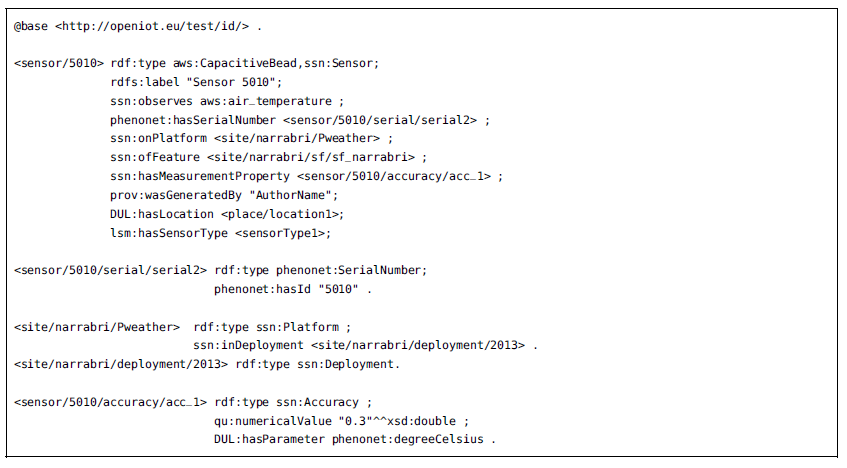
\includegraphics[scale=0.6]{images/semantica_xgsn}
\caption{Sintaxis usada por XGSN.}\label{L304}
\end{figure}

La figura \ref{L305} muestra un registro de un sensor virtual, en el que se almacena una instancia del sensor (metadatos) en la nube.  
Mediante XGSN se envían esos metadatos y ,a través de LSM, se exponen como datos enlazados mediante la representación RDF, para que otros servicios puedan descubrirlo y obtener información.
\begin{figure}[H]
\centering
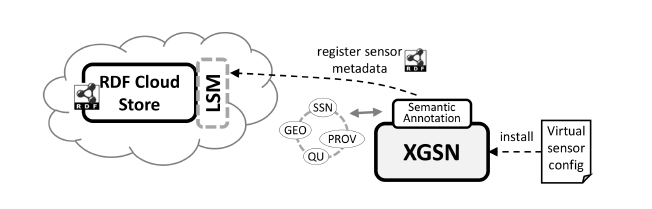
\includegraphics[scale=0.6]{images/registration_sensor_xgsm}
\caption{Registro de un sensor virtual.}\label{L305}
\end{figure}
\subsubsection{Mobile broker}
OpenIoT ofrece soporte para el descubrimiento y recoleccioón de datos por parte de sensores móviles tales como pulseras, gafas, relojes, en definitiva, sensores incluidos en dispositivos móviles. Todo esto se realiza a través de un middleware publish/subscribe para IoT llamado CUPUS (CloUd-based PUblish/Subscribe middleware). \\
CUPUS tiene dos componentes principales: 1) un agente (mobile broker, de ahora en adelante) ejecutándose en un dispositivo móvil y 2) un motor de procesado en la nube basado en publish/subscribe (cloud broker, de ahora en adelante), que se encarga del procesamiento de los datos recopilados por los sensores. CUPUS soporta el contenido basado en publish/subscribe tanto en la nube como en los dispositivos móviles.\\
En la arquitectura OpenIoT, los datos recopilados por los dispositivos móviles se anotan y almacenan en la nube, a través de X-GSN, de la misma forma que con los sensores estacionarios. \\

El mobile broker puede controlar los sensores conectados localmente y realizar un preprocesamiento de los datos adquiridos por los sensores y enviarlos a la nube. Además, también puede recibir publicaciones de la nube y notificar a los clientes que estén subscritos. Como se puede observar en la siguiente figura, el mobile broker recibe los datos de los sensores a través de un mensaje publish y los envía al cloud broker. Pudiendo también conectarse o desconectarse del mismo.\\

El cloud broker puede enviar una notificación al mobile broker. Por otro lado, el cloud broker envía una instancia de los datos del sensor ya procesados al almacenamiento RDF, a través de X-GSN, de la misma forma que en los sensores estacionarios, tal y como se ha visto anteriormente.


\begin{figure}[H]
\centering
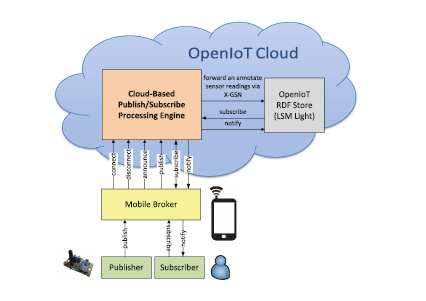
\includegraphics[scale=0.8]{images/mobilebroker_openiot}
\caption{Arquitectura publish/subscribe}\label{L306}
\end{figure}
\subsubsection{Descubrimiento y registro de recursos}
OpenIoT controla el registro y descubrimiento de sensores a través de X-GSN. Cada sensor se tiene que registrar en el LSM y así, otras aplicaciones y usuarios pueden descubrirlo y obtener acceso a sus datos. Los sensores se registran enviando la representación de sus metadatos a través de XGSN. Como se ha visto, XGSN se encarga de crear la sintaxis RDF y enviarla al repositorio. LSM se encarga de exponer esos datos como datos enlazados para que puedan ser compartidos entre sí.
\subsubsection{Autenticación y acceso a los recursos}
La diversidad de aplicaciones interactuando en un entorno IoT hace que la seguridad sea un punto clave para poder proteger los datos. OpenIoT deja la seguridad en manos del servicio CAS (Central authorization service), encargado de la seguridad en la web.\\

La primera vez se redirecciona a los usuarios a la página de login para que se lleve a cabo una autenticación. Si esta autenticación es correcta, el CAS redirecciona al usuario a la pagina web original enviando un token. Este token se envía de un servicio a otro en cada petición y cada servicio se encarga de comprobar la validez del token.

\section{Proyectos}
Hay varios casos de éxito desarrollados mediante la plataforma OpenIoT. Algunos de ellos son Urban Crowdsensing, Phenonet o Silver Angel.
\begin{itemize}
\item[•]\textbf{Urban Crowdsensing}\\
Este proyecto se aplica al medio ambiente. Realiza una monitorización del aire de entornos urbanos. En la figura \ref{L307} se muestra la plataforma OpenIoT sobre la que está construida esta aplicación
\begin{figure}[H]
\centering
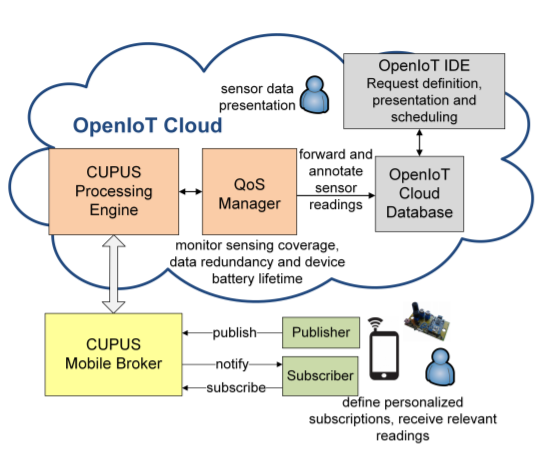
\includegraphics[scale=0.4]{images/crowd_sensing}
\caption{Arquitectura Crowd Sensing}\label{L307}
\end{figure} 

Cualquier dispositivo recoge datos del aire en el ambiente urbano, como por ejemplo, O$_{3}$ , O$_{2}$, CO$_{2}$. Estos datos son enviados a la nube OpenIoT para que sean procesados y filtrados y, posteriormente, reenviados a los smartphones, posibilitando así una monitrización en tiempo real del aire de una ciudad. Pudiendo así, por ejemplo, evitar salir a practicar un deporte en situaciones de alta polución.


\item[•]\textbf{Phenonet}\\
Se aplica en la agricultura. Permite procesar y visualizar datos del terreno en tiempo real. Esto ayuda a los científicos a identificar las plagas de cultivos y así, incrementar la eficiencia y rendimiento en la agricultura. 
\item[•]\textbf{Silver Angel}\\
Tiene una aplicación en la vida diaria de las personas. Está pensada para ayudar a la vida independiente de las personas mayores y, además, para facilitar el encuentro con amigos. Silver Angel permite reunir información de la cantidad de gente que hay en un determinado lugar, que hagan uso de Silver Angel, también reúne información del ruido ambiente o de los niveles de polen del medio ambiente. Así, permite a las personas reunirse dependiendo de sus preferencias; muchas o pocas personas, un alto o bajo ruido...
\\
Silver Angel emite alarmas para ayudar en la vida diaria de personas mayores. Cualquier objeto alrededor de la casa podría avisar de cualquier problema que se haya detectado. Por ejemplo, puede avisar cuando la puerta esté abierta o cerrada o cuando la temperatura de la casa esté por encima o por debajo de un umbral. Si detecta el problema, se envía una alarma a los usuarios que se hayan predefinido.
\end{itemize}

\chapter{OpenIoT}
\section{Introducción}
A pesar de la expansión de las aplicaciones IoT en la nube, la ausencia de una semántica que proporcione una interoperabilidad entre las diferentes aplicaciones es una de las principales limitaciones de IoT. Esta ausencia de una unificación se refleja en los diferentes vocabularios y formas para describir las cosas/objetos físicos. No existe un modelo a seguir para integrar todos los servicios, como sí existe en redes IP. \\

OpenIoT surge como un proyecto europeo que busca la unificación de esas soluciones. Se trata de una plataforma de código abierto que proporciona una convergencia entre los diversos sistemas IoT. Mezcla el concepto Cloud-Computing con el concepto de redes de sensores de IoT.\\ 

OpenIoT se basa en SSN como el modelo para la unificación de los diferentes sistemas IoT y flujo de datos. OpenIoT ofrece una infraestructura versátil para coleccionar datos de cualquier sensor disponible. Se hace uso del concepto "datos enlazados", Linked Data en inglés. En el que los datos de los sensores se vinculan entre sí, para que puedan ser compartidos y entenderse entre ellos, ampliando así la información. OpenIoT incluye también un middleware que facilita la recolección de datos de cualquier sensor disponible.
\section{Plataforma}
\subsection{Arquitectura}
La arquitectura de la plataforma se puede ver en la figura \ref{L400} 
\begin{figure}[H]
\centering
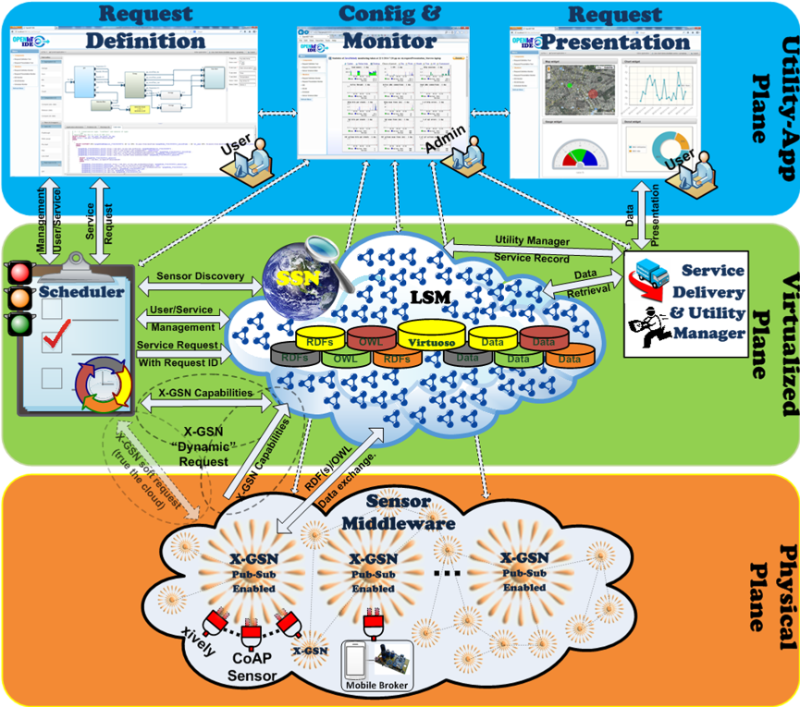
\includegraphics[scale=0.4]{images/openiot_platform1}
\caption{Arquitectura OpenIoT}\label{L400}
\end{figure}
\subsubsection*{Plano físico}
En el plano físico se encuentran los sensores. En OpenIoT se usa X-GSN como middleware para el intercambio de información entre los sensores y la nube. Este middleware se encarga de filtrar, combinar y coleccionar los datos recopilados por los sensores. X-GSN es una versión extendida de GSN, cuya principal característica es el uso de sensores virtuales. Los datos de los sensores están escritos basándose en SSN (Semantic Sensor Network), una semántica para las redes de sensores. Esto proporciona una representación que hace más fácil compartir, descubrir, integrar e interpretar los datos. Un ejemplo de esta semántica se puede ver en la figura \ref{L401} \\
\begin{figure}[H]
\centering
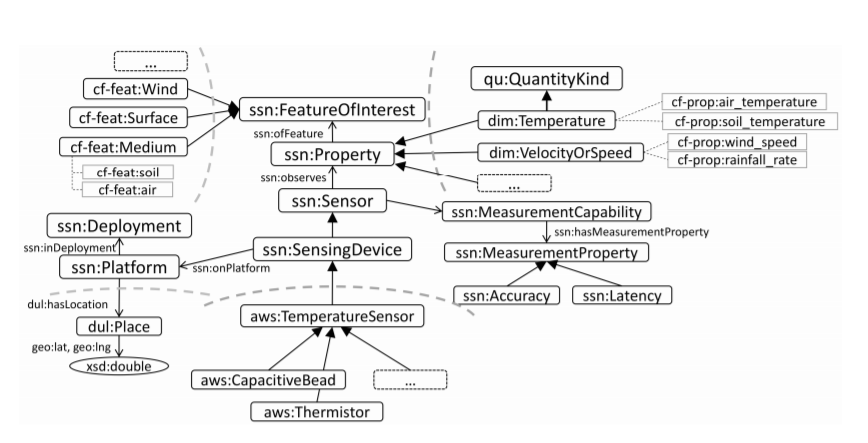
\includegraphics[scale=0.4]{images/ssn_capture}
\caption{Semántica de SSN.}\label{L401}
\end{figure}
En X-GSN se configuran los sensores usando una descripción en XML, en la que se definen los campos de los sensores. Estos campos están asociados a la semántica SSN. En la figura \ref{L404} se puede ver un ejemplo de esta descripción. \\
Para realizar el registro de sensores en la plataforma OpenIoT, es necesario que cada sensor tenga una instancia del mismo almacenada en la nube. Este registro se realiza mediante el envío a la plataforma LSM de un archivo de los metadatos del sensor, en el que se definen las propiedades del mismo. Un ejemplo de este archivo se puede ver en la figura \ref{L402}.
\begin{figure}[H]
\centering
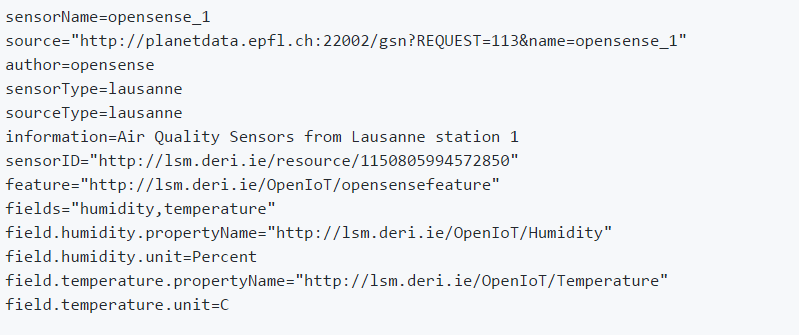
\includegraphics[scale=0.4]{images/metadata_capture}
\caption{Metadatos de un sensor.}\label{L402}
\end{figure}
mediante un archivo XML enviado a la plataforma LSM. En este XML se usa una descripción en formato RDF
Los sensores, situados en el plano físico, envían una instancia de sus datos (situación geográfica, memoria...) a la nube. Estos metadatos se envían en formato RDF, una semántica usada en la Web enlazada ("Linked Web", en inglés) y así pueden conectar con LSM.\\

En la figura \ref{L403} se puede ver el proceso para el registro de un sensor en OpenIoT. Inicialmente se crea y se configura el sensor, mediante la descripción XML. Un ejemplo de esta descripción se puede ver en la figura \ref{L404}. Posteriormente se envía un archivo a la plataforma LSM en la nube conteniendo las propiedades del sensor. Éste se transforma en una descripción RDF, una descripción usada en la Web Semántica, que permite una representación de datos enlazados, lo que facilita el descubrimiento de recursos.
\begin{figure}[H]
\centering
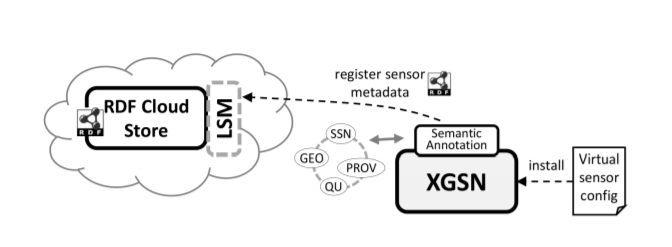
\includegraphics[scale=0.4]{images/registration_capture}
\caption{Registro de un sensor virtual}\label{L403}
\end{figure}
\begin{figure}[H]
\centering
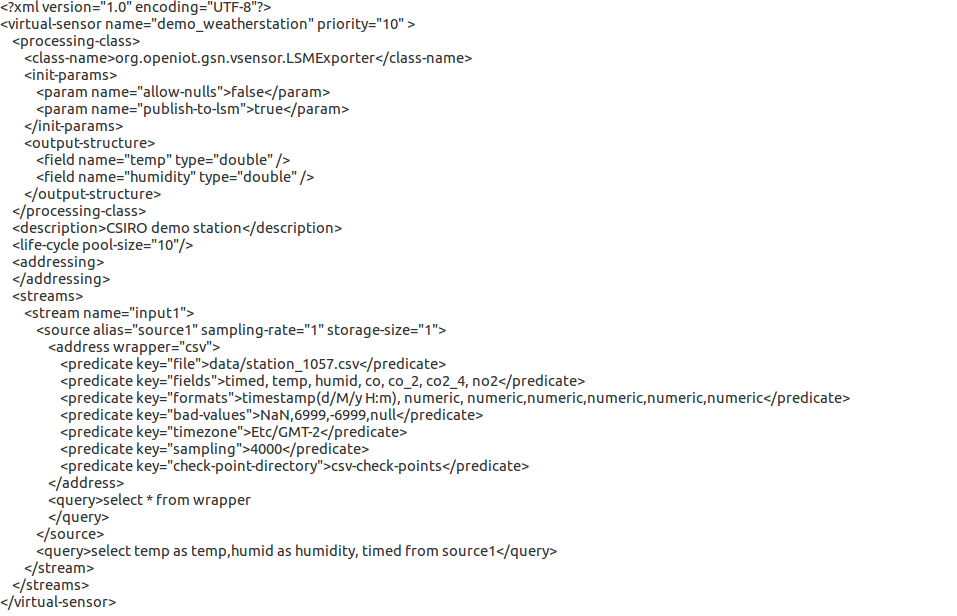
\includegraphics[scale=0.5]{images/configuration_capture}
\caption{Configuración de un sensor.}\label{L404}
\end{figure}
OpenIoT ofrece soporte para el descubrimiento y recoleccioón de datos por parte de sensores móviles tales como pulseras, gafas, relojes, en definitiva, sensores incluidos en dispositivos móviles. Todo esto se realiza a través de un middleware publish/subscribe para IoT llamado CUPUS (CloUd-based PUblish/Subscribe middleware). \\
CUPUS tiene dos componentes principales: 1) un agente (mobile broker, de ahora en adelante) ejecutándose en un dispositivo móvil y 2) un motor de procesado en la nube basado en publish/subscribe (cloud broker, de ahora en adelante), que se encarga del procesamiento de los datos recopilados por los sensores. CUPUS soporta el contenido basado en publish/subscribe.\\
En la arquitectura OpenIoT, los datos recopilados por los dispositivos móviles se anotan y almacenan en la nube, a través de X-GSN, de la misma forma que con los sensores estacionarios. \\

El mobile broker puede controlar los sensores conectados localmente y realizar un preprocesamiento de los datos adquiridos por los sensores y enviarlos a la nube. Además, también puede recibir publicaciones de la nube y notificar a los clientes que estén subscritos. Como se puede observar en la figura \ref{L405}, el mobile broker recibe los datos de los sensores a través de un mensaje publish y los envía al cloud broker. Pudiendo también conectarse o desconectarse del mismo.\\

El cloud broker puede enviar una notificación al mobile broker. Por otro lado, el cloud broker envía una instancia de los datos del sensor ya procesados al almacenamiento RDF, a través de X-GSN, de la misma forma que en los sensores estacionarios, tal y como se ha visto anteriormente.

\begin{figure}[H]
\centering
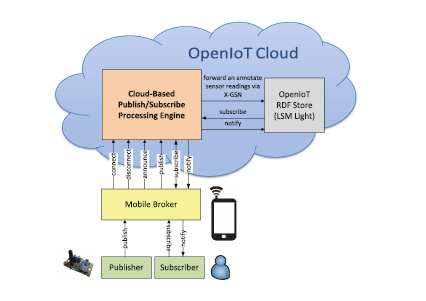
\includegraphics[scale=0.9]{images/mobilebroker_openiot}
\caption{Arquitectura publish/subscribe}\label{L405}
\end{figure}
\subsubsection*{Plano Virtual}
El plano virtual está compuesto por el almacenamiento en la nube (LSM-Light), el Scheduler y el servicio de entrega. \\

LSM-Light (Linked Sensor Middleware Light) es el componente principal de OpenIoT. Es la infraestructura de almacenamiento en la nube. Esta infraestructura, además de almacenar datos y metadatos, también es capaz de ofrecer computación en la nube (software) como por ejemplo Scheduler y SD\&UM.\\ LSM considera los sensores como fuentes de entrada de datos. Los datos provenientes de los sensores se transforman en una representación de datos enlazados, como por ejemplo, RDF. Existen dos formas de importar datos en LSM, pull y push. Una es la fuente de datos (X-GSN,CoAP...) la que se encarga de enviar los datos y la otra es el propio LSM quien obtiene los datos periódicamente. LSM está compuesto por dos módulos, LSM-Client y LSM-Server\\

OpenIoT usa Virtuoso, un middleware y motor de almacenamiento, que combina RDF, XML y base de datos virtuales en un solo sistema. Es el corazón de LSM-Light. \\

El scheduler se encarga de formular las peticiones realizadas por los usuarios y de acuerdo con ellas interactúa con la plataforma OpenIoT a través de la base de datos en la nube. El Scheduler tiene dos funciones prncipales: descubrir sensores y controlar los servicios. Todo esto se realiza mediante peticiones a la BBDD. Las peticiones se realizan en lenguaje SPARQL, un lenguaje usado en la web semántica para consulta de sentencias RDF. En la figura \ref{L406} se observa la Cloud DB junto con cada uno de los servicios que realiza peticiones. Request presentation y Request Definition realizan las peticiones a través de otros servicios (Scheduler y SD\&UM).\\

El servicio Request Definition es quien realiza las peticiones al Scheduler para que éste las procese. La forma que tiene de enviar las peticiones es mediante una API, especificada en la documentación.\\
El SD\&UM (Service Delivery \& Utility Manager), al igual que el Scheduler, realiza peticiones a la Cloud DB mediante una API.
\begin{figure}[H]
\centering
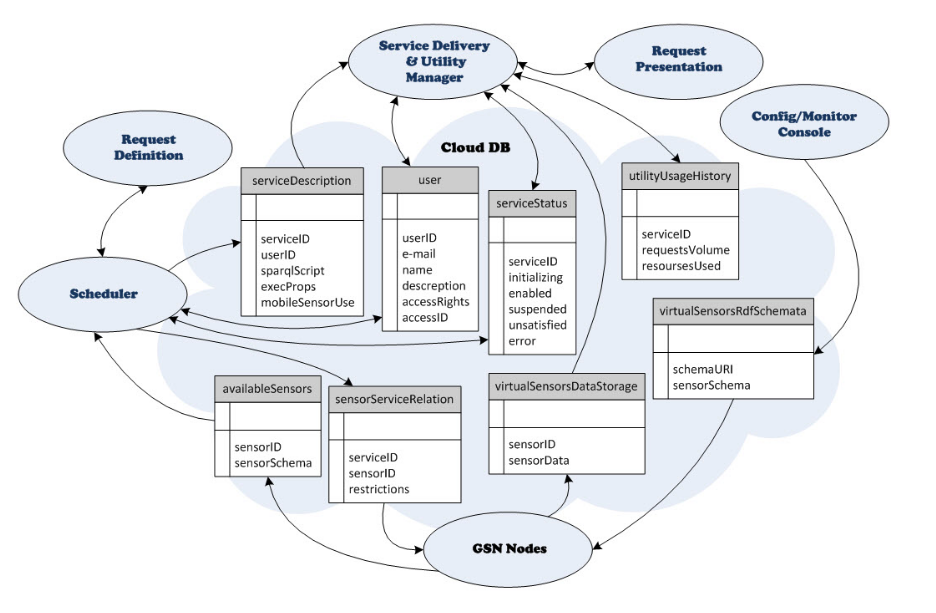
\includegraphics[scale=0.4]{images/cloud_capture}
\caption{Relación de cada servicio con la Cloud DB}\label{L406}
\end{figure}
\subsubsection*{Plano de utilidad}
En este plano se sitúan las interfaces de usuario. 
Request Definition es una aplicación que permite a los usuarios visualizar sus servicios de OpenIoT usando una interfaz basada en nodos. Cada modelo de grafos se divide en aplicaciones, siendo cada una de estas aplicaciones un conjunto de servicios que describen a la aplicación. Esto le permite al usuario controlar diferentes aplicaciones desde un solo punto. Todos estos servicios se almacenan en el Scheduler y se cargan automáticamente cuando el usuario accede a la web. Un ejemplo de esta interfaz se muestra en la figura \ref{L407}

\begin{figure}[H]
\centering
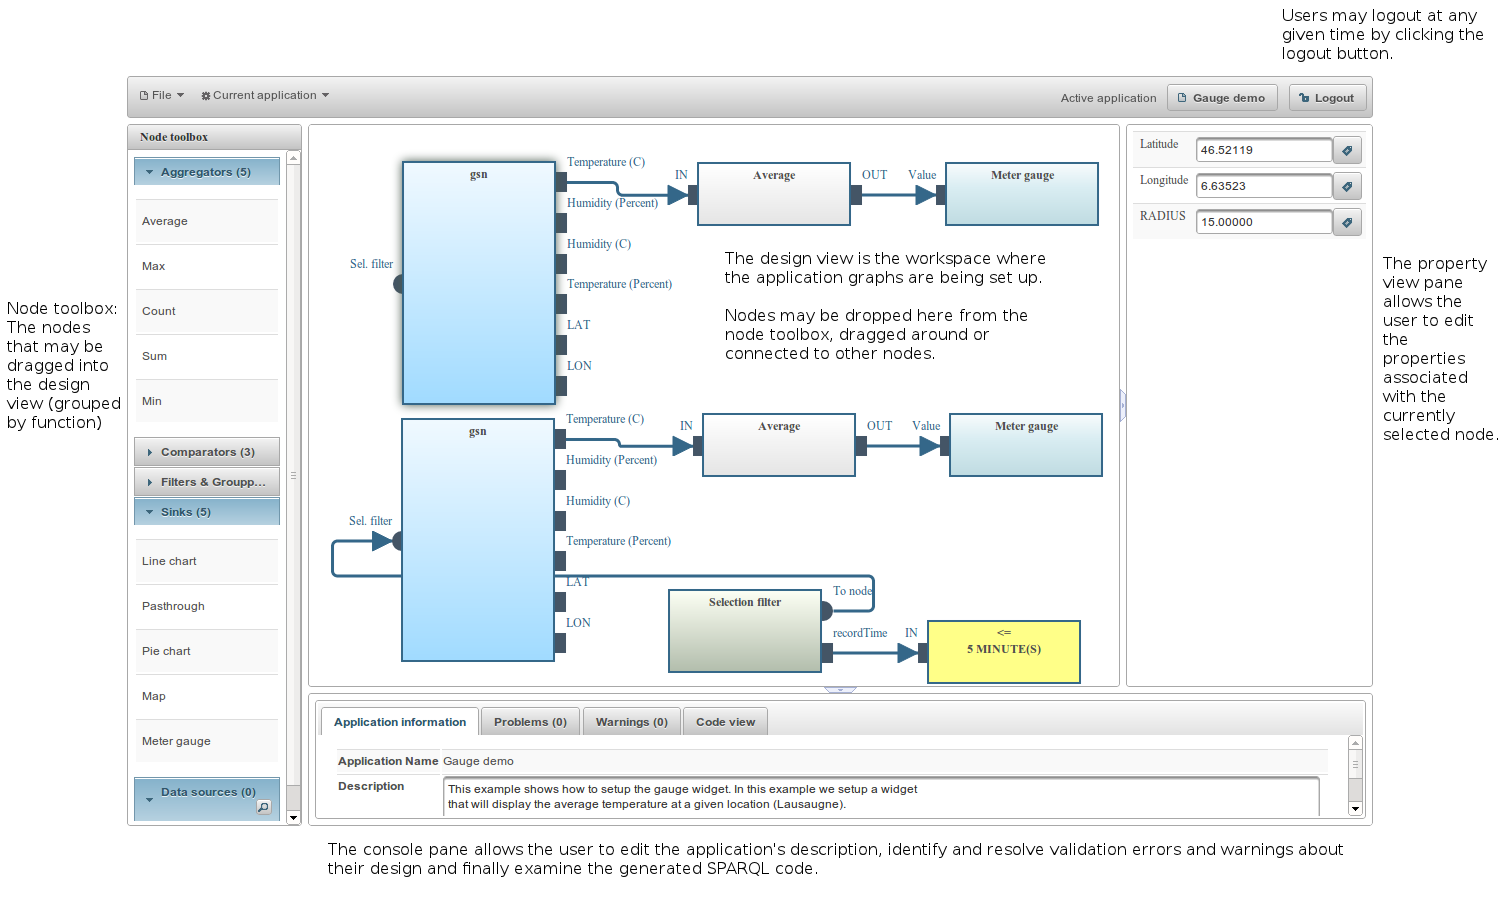
\includegraphics[scale=0.3]{images/requestDefinition}
\caption{Request Definition}\label{L407}
\end{figure}
Request Presentation es una aplicación web que proporciona al usuario una interfaz visual de los servicios que previamente ha creado en Request Definition. Obtiene la información de los nodos de Request Definition y muestra una interfaz con los datos. \\
En la figura \ref{L408} se muestra un ejemplo con la definición del servicio en Request Definition, y en la figura \ref{L409} la interfaz gráfica de los datos en Request Presentation, una vez recopilados.
\begin{figure}[H] 
\hfill
\begin{minipage}[t]{.45\textwidth}
\begin{center}
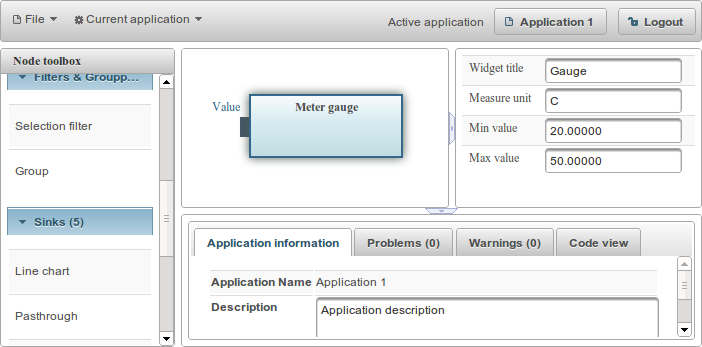
\includegraphics[width=190pt]{images/temperature_definition}
\caption{Definition}
\label{L408}
\end{center}
\end{minipage}
\hfill
\begin{minipage}[t]{.45\textwidth}
\begin{center}
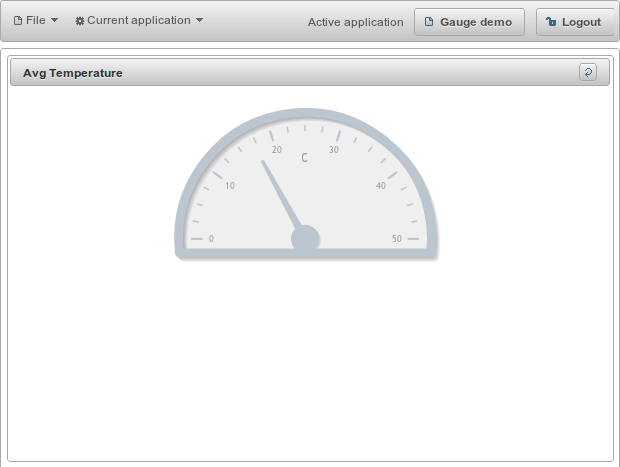
\includegraphics[width=190pt]{images/temperature_presentation}
\caption{Presentation}
\label{L409}
\end{center}
\end{minipage}
\hfill
\end{figure}

El IDE es el otro de los servicios situados en el plano de utilidad. Proporciona accesibilidad a los otros módulos o servicios de OpenIoT.
Otra de las funcionalidades que soporta IDE es la monitorización. Para implementar dicha funcionalidad se usa JavaMelody. Entre las funciones de monitorización se encuentra proporcionar datos sobre el tiempo medio de respuesta o el número de ejecuciones, la toma de decisiones ante problemas o, mostrar gráficos sobre número de sesiones, consumo de java o número de ejecuciones.

\subsection{Flujo de datos}
En base a la arquitectura que se muestra en la figura \ref{L301}, la figura \ref{L0420} representa un ejemplo del flujo que siguen los datos en la plataforma. \\
X-GSN publica los datos de los sensores virtuales basados en la configuración local de cada nodo (sensor). Paso 0. \\
Los usuarios realizan peticiones al Scheduler (paso 1) de los sensores disponibles con determinados atributos usando la interfaz Request Definition.\\
El Scheduler ejecuta (paso 2) estas peticiones (en lenguaje SPARQL) enviadas por los usuarios.\\
Una vez que tenga la respuesta (los sensores disponibles) se envía de vuelta al Scheduler (paso 3) y éste la reenvía al módulo Request Definition (paso 4), mostrándose la información al usuario.\\
El usuario, con ayuda de Request Definiton, define peticiones para  realizar determinadas reglas sobre los sensores analizados. Esta información se guarda en un objeto OSDSpec (Figura \ref{L0421}). Este objeto se envía entonces al Scheduler con la ayuda de 'registerService (paso 5).\\
El Scheduler analiza la información recibida y envía la petición al servicio necesario (paso 6).\\
Una vez que se haya configurado, el usuario puede usar el módulo Request Presentation para visualizar los datos del servicio registrado.\\
Con ayuda del SD\&UM 'getAvailableAppIDs' el Request Presentation (pasos 7,8,9 y 10) recupera todos los servicios/aplicaciones registrados de acuerdo a un usuario específico\\\
El usuario realiza una petición para recuperar los resultados relacionados con el servicio en concreto. Esto se hace enviando una petición ("pollForReport") desde Request Presentation al SD\&UM pasándole el ID de la aplicación ('application ID') (paso 11).\\
El SD\&UM realiza una petición ("getService") (paso 12) para solicitar toda la información relacionada al servicio.\\
El servicio proporciona la información al SD\&UM (paso 13).\\
El SD\&UM analiza la información, disponible en un objeto OSMO, y reenvía el script SPARQL incluido, el cual ha sido creado por Request Definition (paso 5) y almacenado por el Scheduler (paso 6), a la interfaz SPARQL del servicio (paso 14).\\
El resultado se envía al SD\&UM (paso 15) en formato SparqlResultsDoc\\El SD\&UM lo reenvía al Request Presentation (paso 16) en un objeto que incluye información de cómo esos datos se deben presentar (Figura \ref{L0422}).

\begin{figure}[H]
\centering
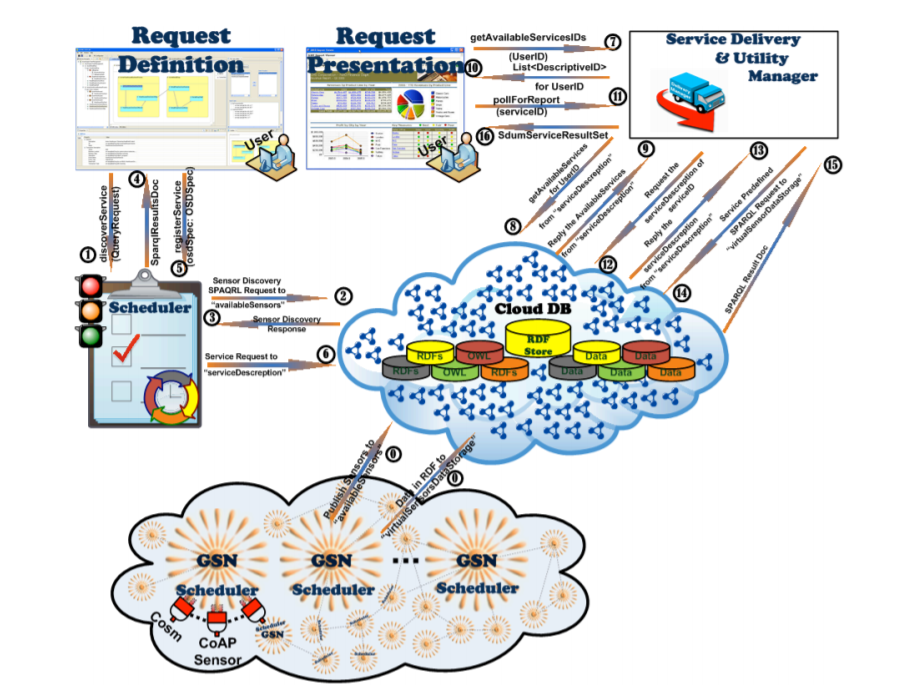
\includegraphics[scale=0.5]{images/dataFlow_capture}
\caption{Flujo de datos en OpenIoT}\label{L0420}
\end{figure}

\begin{figure}[H]
\centering
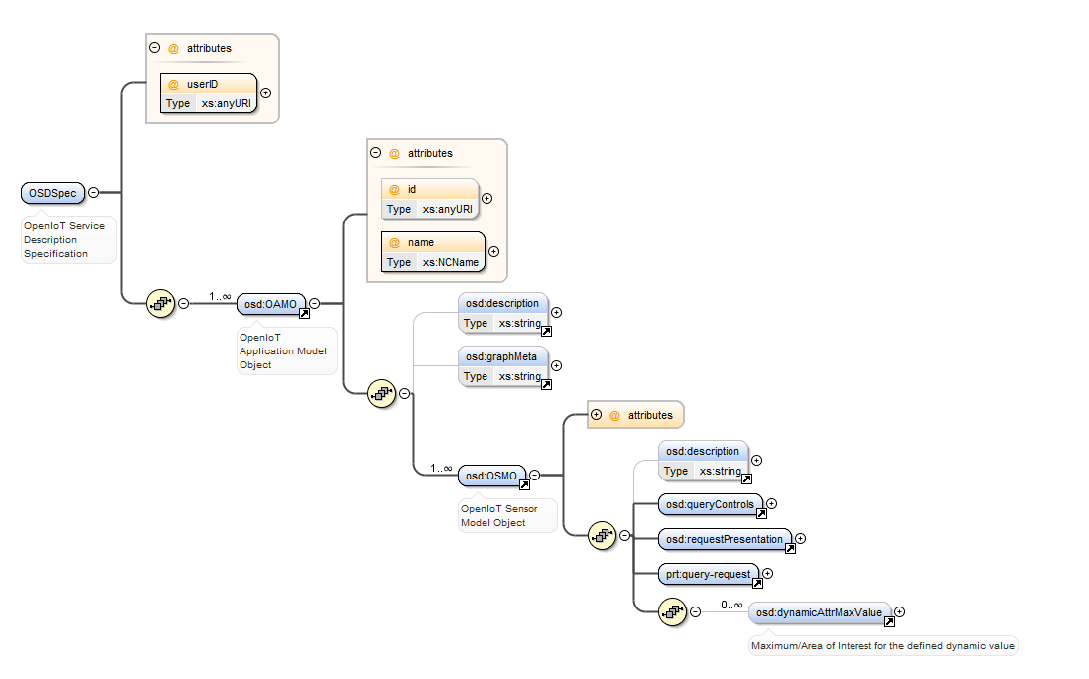
\includegraphics[scale=0.5]{images/osd_sdum}
\caption{Grafo de un objeto OSDSpec.}\label{L0421}
\end{figure}

\begin{figure}[H]
\centering
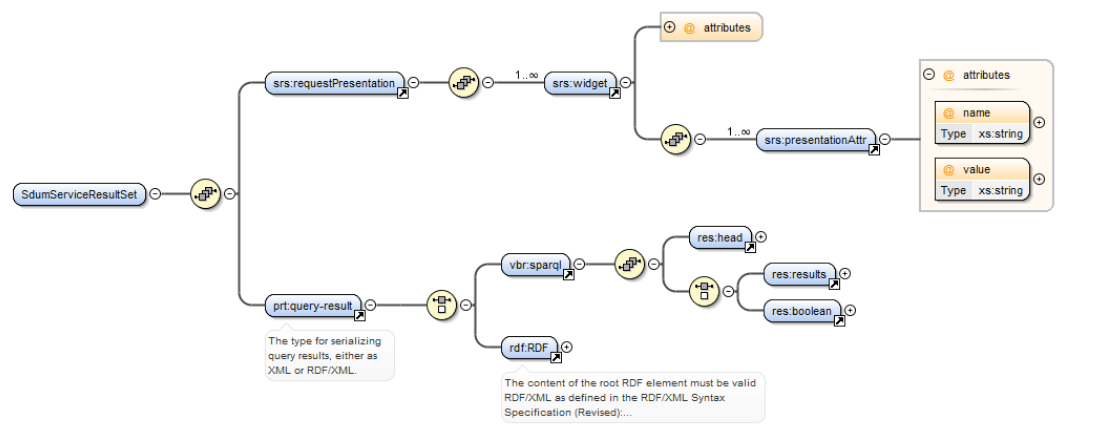
\includegraphics[scale=0.5]{images/sdum_service}
\caption{Grafo de un objeto SdumServiceResultSet.}\label{L0422}
\end{figure}
\subsection{Uso de la plataforma}
...
\subsubsection*{Ventajas}
En IoT cualquier cosa u objeto (TV,Smartphone...) genera una gran cantidad de eventos. Cada uno de estos objetos usa tecnologías diferentes y, desarrollar aplicaciones y servicios para controlar todo esto puede llegar a ser una tarea muy complicada. Por ello, se usan middlewares con el fin facilitar el desarrollo proporcionando una integración entre la comunicación y la computación de los dispositivos. Entre los middleware se encuentra MAPS, TinyDB o MQTT, mencionado anteriormente.\\

A pesar de que con los middleware se facilita el desarrollo de aplicaciones en IoT, cada middleware cumple una serie de requisitos que puede que no sirvan para una determinada aplicación. Por ejemplo, en este caso, MQTT no cumplía alguno de los requisitos exigidos. No hay un middleware que reúna todas necesidades exigidas. Es aquí donde aparece OpenIoT, que permite reunir los servicios en una única plataforma.\\

La principal ventaja de OpenIoT es la unificación de los diferentes sistemas o servicios IoT, así como el envío de datos.\\

A través de la herramienta IDE (Integrated Development Environment) Core (figura \ref{L0421} ) que ofrece OpenIoT, se puede controlar las aplicaciones IoT. Esta herramienta integra muchas de las herramientas de OpenIoT en una. Permite configurar los sensores para su integración en X-GSN (Schema Editor), monitorización del estado de los servicios IoT (SDUM) o definir los servicios IoT (Request Definition). Esto permite el desarrollo de aplicaciones IoT de una manera más rápida y sencilla.\\


\begin{figure}[H]
\centering
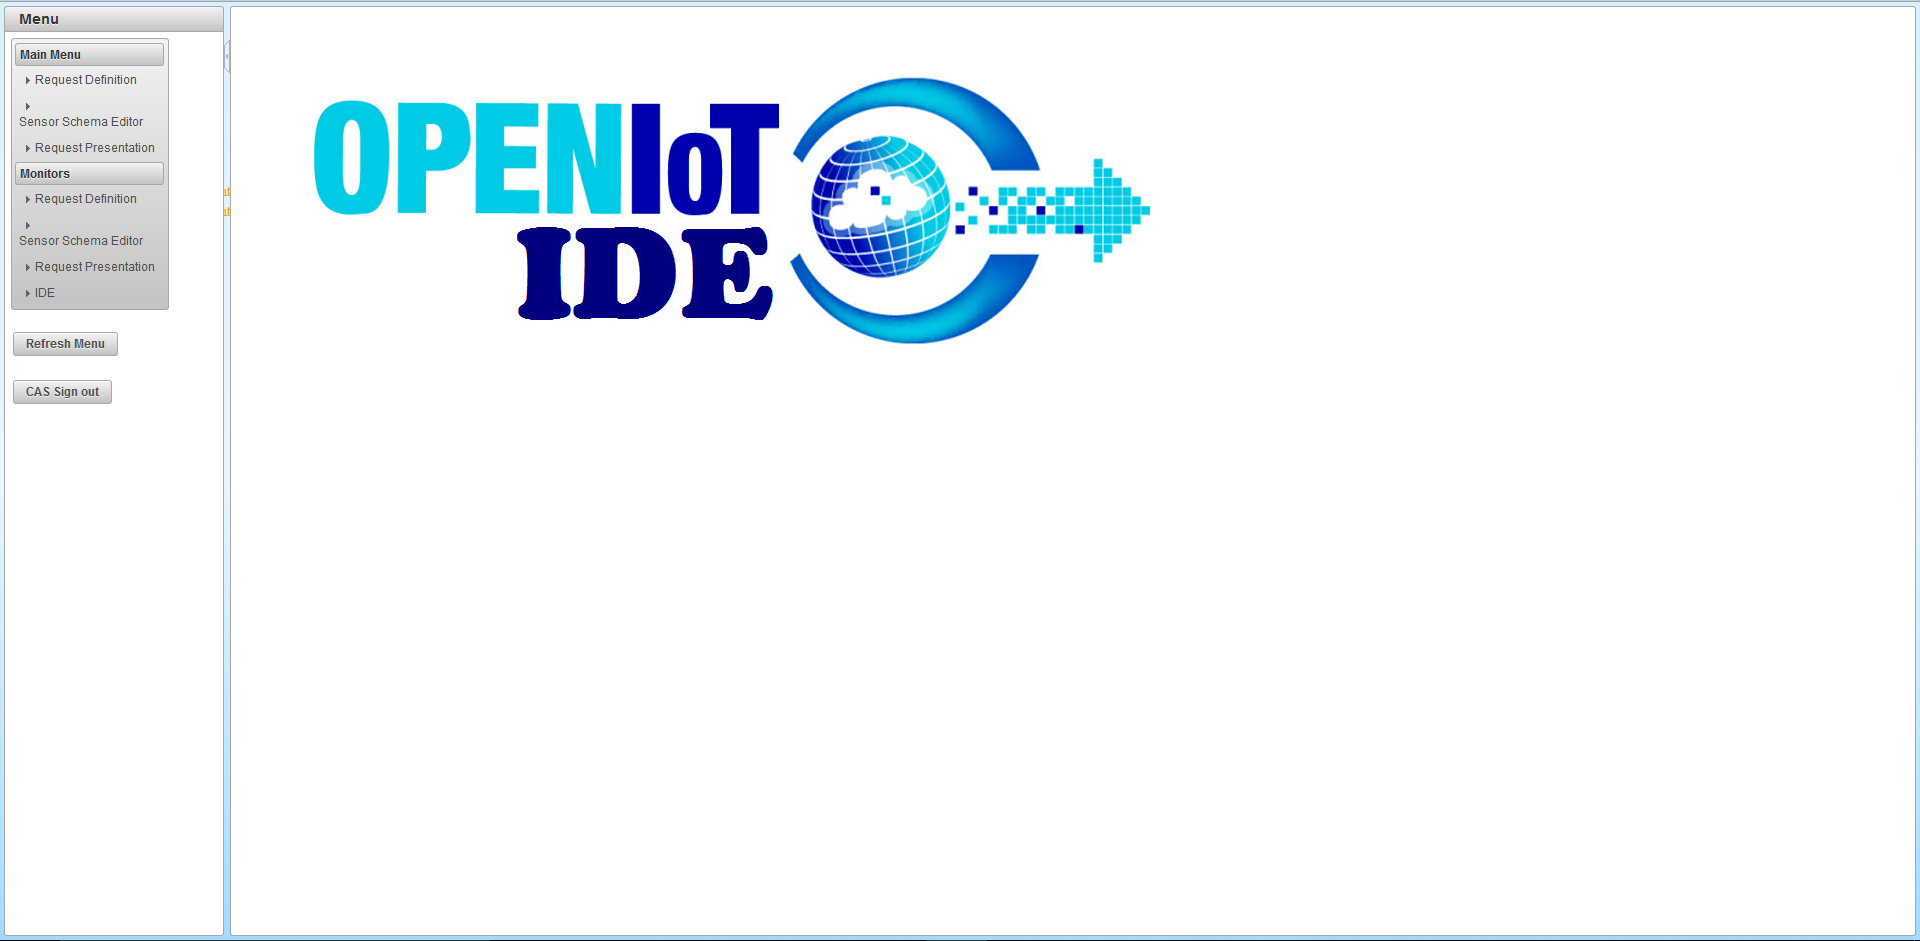
\includegraphics[scale=0.3]{images/idecore_figure}
\caption{OpenIoT IDE}\label{L0421}
\end{figure}

\begin{figure}[H]
\centering
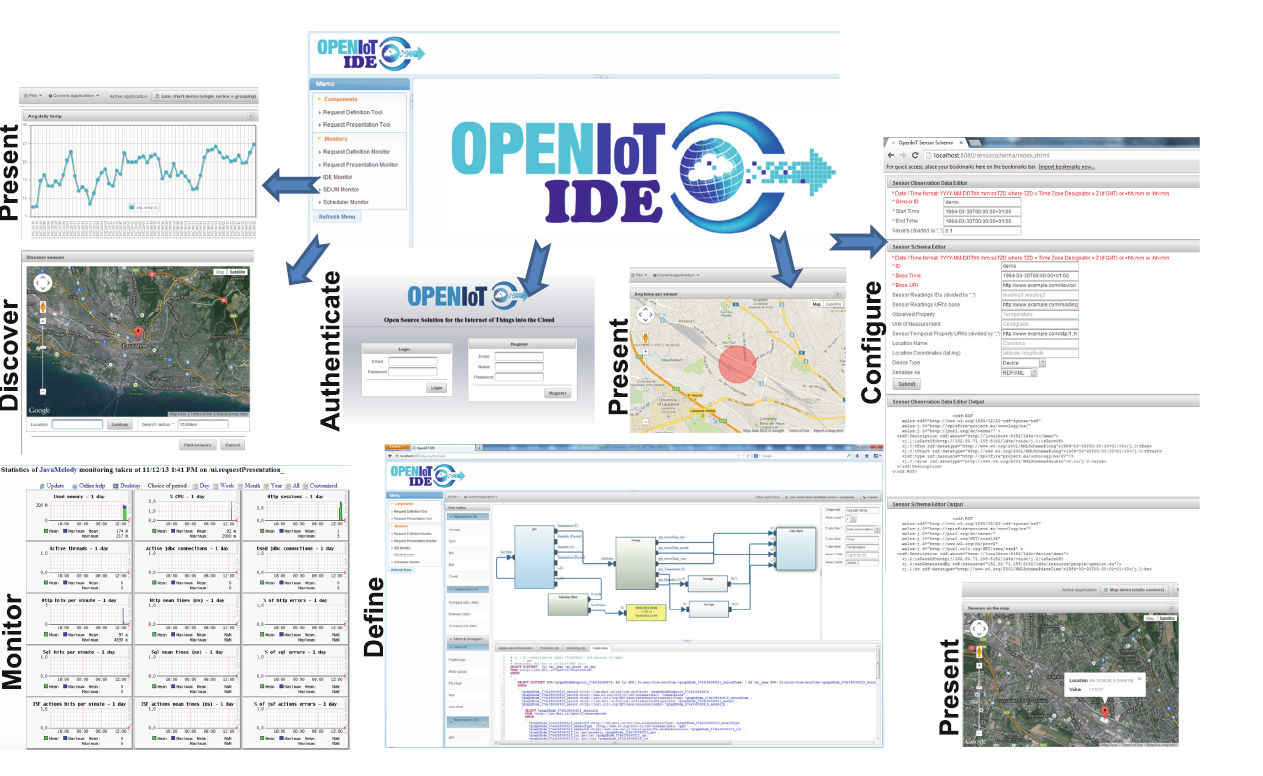
\includegraphics[scale=0.55]{images/idecoretools_capture}
\caption{Servicios integrados en IDE}\label{L0421}
\end{figure}

\subsection{Requisitos}
Las aplicaciones IoT deben cumplir una serie de requisitos, algunos de ellos necesarios en un entorno IoT. Algunos de estos requisitos son:

\subsubsection*{Escalabilidad}
OpenIoT es una plataforma totalmente escalable debido a la característica de descubrimiento de recursos que posee. Se pueden añadir nuevos nodos tan solo configurando el sensor y enviando la información sobre sus datos (metadatos) al almacenamiento en la nube. Una vez registrado el sensor, el usuario puede acceder al nuevo nodo (sensor).
\subsubsection*{Disponibilidad}
OpenIoT está formado por varios módulos/servicios, cuyo funcionamiento es responsable del funcionamiento global de la plataforma. Por ello, un fallo en alguno de los servicios (i.e el Scheduler), implica un fallo en la plataforma. 
Debido a esta dependencia, se puede decir que OpenIoT no dispone de una gran disponibilidad.
\subsubsection*{Seguridad}
La diversidad de aplicaciones interactuando en un entorno IoT hace que la seguridad sea un punto clave para poder proteger los datos. OpenIoT deja la seguridad en manos del servicio CAS (Central authorization service), encargado de la seguridad en la web.\\

La primera vez se redirecciona a los usuarios a la página de login para que se lleve a cabo una autenticación. Si esta autenticación es correcta, el CAS redirecciona al usuario a la pagina web original enviando un token. Este token se envía de un servicio a otro en cada petición y cada servicio se encarga de comprobar la validez del token.
\begin{figure}[H]
\centering
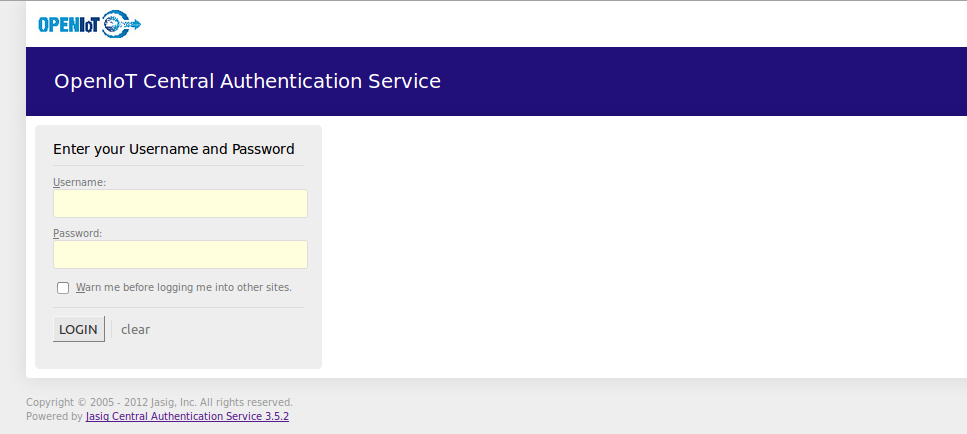
\includegraphics[scale=0.5]{images/login_capture}
\caption{Login en CAS}\label{L410}
\end{figure}
La seguridad en OpenIoT se divide en 3 módulos:
\begin{itemize}
\item[•]\textbf{Security Server:} En este módulo se usa CAS para la autenticación y autorización. Sus datos se almacenan en LSM-server. Cada cliente se tiene que registrar en CAS.
\item[•] \textbf{Security Client:} Este modulo proporciona control de acceso y autenticación. Se puede usar en aplicaciones web que interactuan con los usuarios.  
\item[•] \textbf{Security Management:} Se trata de un módulo que se usa para llevar un control sobre servicios, usuarios y permisos.
\end{itemize}
\subsubsection*{Descubrimiento de recursos}
Una de las características principales de OpenIoT es el descubrimiento de recursos. Una vez que los sensores envían su configuración a la nube a través de X-GSN, OpenIoT mediante el Scheduler, haciendo uso de la semántica SSN, es capaz de descubrir nuevos sensores o nodos.
\subsubsection*{Control de recursos}
OpenIoT, a través de la herramienta SDUM, permite llevar una constante monitorización sobre los recursos. Esto permite, además de la recopilación y visualización de los datos, llevar un control de los recursos.  
\subsubsection*{Tiempo real}
OpenIoT proporciona un servicio en tiempo real. El usuario a través de las interfaces de usuario puede realizar un seguimiento en tiempo real de los datos recopilados por los sensores.
\subsubsection*{Interoperabilidad}
La interoperabilidad de los servicios IoT es la idea fundamental por la que surgió OpenIoT. Se buscaba unificar distintos servicios en una única plataforma. En OpenIoT se unifica todo lo relacionado con redes de sensores (Middleware...) y lo relacionado con el Cloud Computing (base de datos, herramientas de procesamiento...).
\subsubsection*{Distribuido}


\subsection{Caso práctico}

\subsection{Casos de éxito con la plataforma}
Entre quién ha desplegado la plataforma con éxito se encuentra:
\begin{itemize}
\item[•] Universidad nacional de Irlanda - DERI
\item[•] Universidad de Zagreb - FER
\item[•] SENSAP S.A
\item[•] CSIRO
\item[•] Universidad de Estambul
\end{itemize}
\subsubsection{OpenIoT en la industria}
Cada vez más, en la industria se instalan un gran número de sensores para controlar el proceso de producción de una planta. Estos sensores generan un gran volumen de datos por lo que es necesario una solución para capturar, almacenar y procesar esos datos. SENSAP S.A (www.sensap.eu) ha desarrollado una solución basada en OpenIoT para la monitorización y seguimiento del flujo de materiales en un proceso de producción. Le permite definir y visualizar dinámicamente los KPIs (indicadores de rendimiento en la industria). En este entorno, los KPIs son el flujo de datos necesarios, los cuales son: A)recopilados por sensores físicos situados en la planta, B)transformados en el modelo de datos EPC-IS, un estándar usado en la industria, C) transmitidos al middleware X-GSN que asegura una anotación semántica de estos datos y su posterior publicación a la nube OpenIoT. Los sensores virtuales son capaces de calcular entre otros: \\
\begin{itemize}
\item[•] Tasa de operación para un proceso específico
\item[•] Métricas de utilización de las maquinas
\item[•] Tasa de producción por tipo de producto
\item[•] Porcentaje de tiempo una operación que ha sido completada
\end{itemize} 

Una vez que se publica la información a la nube, los fabricantes son capaces de obtener y sintetizar la información de los sensores virtuales, con el fin de calcular los KPIs para los determinados procesos.\\

Para llevar a cabo este proyecto, se usó la siguiente implementación:\\
\begin{itemize}
\item[•] Sensores: Sensores físicos con el fin de calcular KPIs (tasas de operación, información de calidad...). Sensores ópticos, escáneres de códigos de barras, son algunos de los sensores utilizados en este proyecto.
\item[•] S-BOX: Productos propios desarrollados por SENSAP, para coleccionar datos de los sensores y transformarlos en eventos EPC-IS, asociados a los procesos de fabricación.
\item[•] X-GSN: Ese flujo de datos EPC-IS se envía al middleware X-GSN. Siguiendo el proceso de OpenIoT, el middleware X-GSN convierte ese flujo de datos en la anotación SSN.
\item[•] LSM: La información KPIs se envía a la nube (LSM Cloud) a través de X-GSN, tal y como marca el proceso de OpenIoT
\item[•] Visualización: Usando la herramienta Request Definition de OpenIoT, se definen servicios que calculan los KPIs asociados al proceso de fabricación. Este cálculo lo realiza a partir de los datos disponibles en el LSM Cloud. 
\end{itemize}
\subsubsection{OpenIoT en la agricultura}
Otros de los proyectos en los que se ha usado OpenIoT ha sido Phenonet, desarrollado por CSIRO. Se trata de un proyecto usado en la agricultura que permite procesar y visualizar datos del terreno en tiempo real. Esto ayuda a la toma de decisiones sobre el cultivo como, por ejemplo, planificar los recursos de agua o de nitrógeno en el cultivo y así, incrementar la eficiencia y rendimiento. La arquitectura de Phenonet se puede ver en la figura \ref{L411}
\begin{figure}[H]
\centering
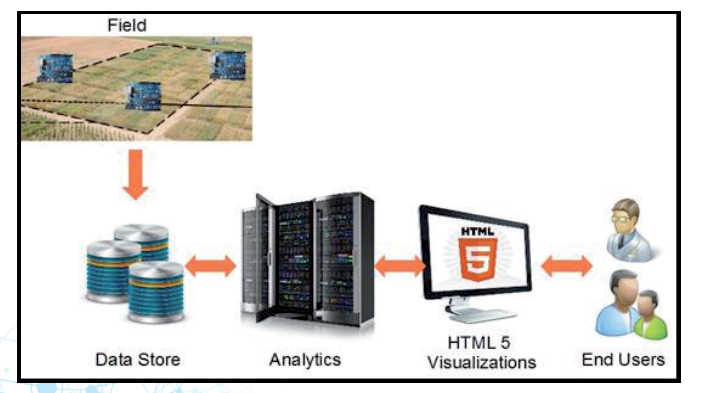
\includegraphics[scale=0.4]{images/phenonet_capture}
\caption{Arquitectura de Phenonet}\label{L411}
\end{figure}

En el campo ('field') se sitúan los sensores para medir temperatura, humedad o velocidad del viento entre otros. Los datos y metadatos se almacenan y posteriormente se procesan y analizan mediante el componente 'Data analysis'. A este componente se accede a a través de una API mediante HTML. Phenonet está basado en los siguientes módulos de OpenIoT:
\begin{itemize}
\item[•] X-GSN: Se encarga de los dato provenientes del Data Store/Field.
\item[•] Scheduler y SD\&UM: Usado para construir un experimento Phenonet en OpenIoT.
\item[•] LSM-Light: Se almacenan los datos existentes en Data Store para poder permitir el descubrimiento de sensores.
\item[•] Request Definition y Presentation: Estas herramientas se usan para el diseño. 
\end{itemize}

\chapter{KAA}
\section{Arquitectura}
Kaa es un middleware de código abierto que, al igual que OpenIoT, busca un control e integración de las aplicaciones IoT. Kaa tiene un poderoso back-end que facilita el desarrollo de aplicaciones en un entorno IoT. Kaa soporta múltiples plataformas en el lado del cliente, mediante puntos finales (SDKs), en diferentes lenguajes de programación. El SDK es una librería 'empotrada' en el dispositivo conectado. Esto, junto con un lenguaje de definición de datos ("data schema"), hace que Kaa sea una plataforma muy rápida y flexible. Kaa ha sido diseñada como una plataforma robusta y fácil de usar.\\ En la figura \ref{L501} se puede ver su arquitectura.\\
Un cluster Kaa representa un número de nodos (Kaa server) interconectados. La figura \ref{L502} muestra un flujo de datos común, donde se puede ver un cluster Kaa, formado por un kaa server.  



\textbf{Nota: La versión de la plataforma analizada en este documento ha sido la 0.10, la última hasta la fecha.}

/////////////////Palabras clave: CLUSTER,SDK,NODE,SCHEMA,LOG////////////
\begin{figure}[H]
\centering
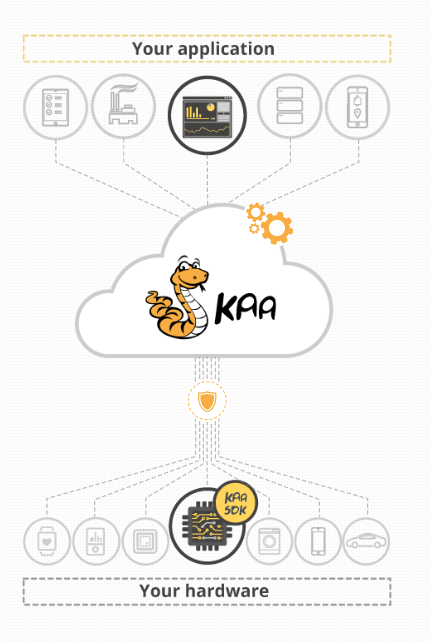
\includegraphics[scale=0.5]{images/kaa_platform}
\caption{Arquitectura Kaa}\label{L501}
\end{figure}
Un conjunto de nodos interconectados representa un Cluster Kaa. Un Cluster requiere bases de datos SQL y NoSQL para almacenar los datos y metadatos de los endpoints. El servidor Kaa usa Apache Zookeeper para coordinar los servicios.
\begin{figure}[H]
\centering
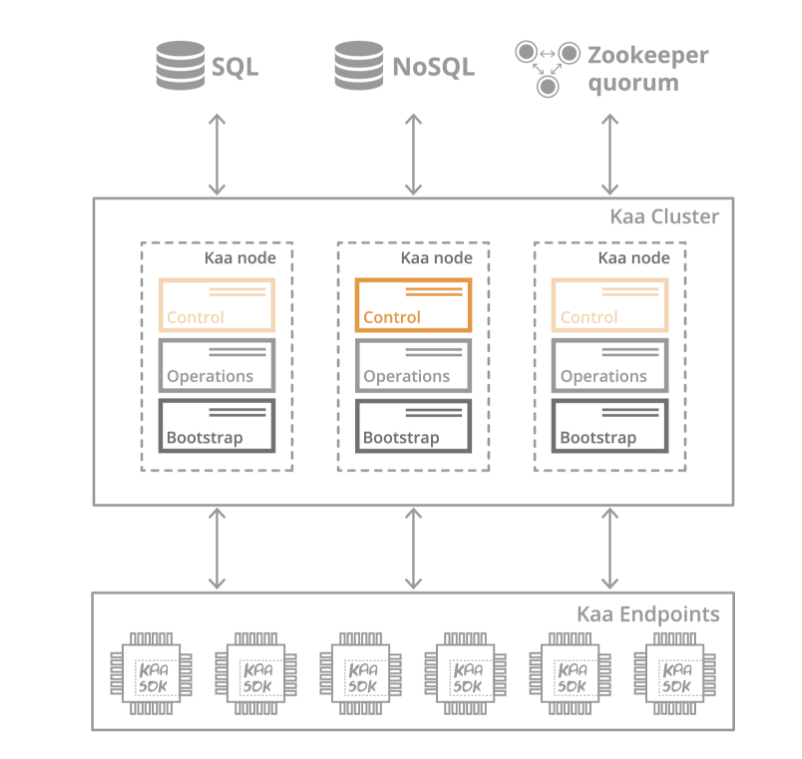
\includegraphics[scale=0.6]{images/arquitectura_kaa}
\caption{Cluster Kaa}\label{L501}
\end{figure}
Un nodo en un cluster está ejecutando una combinación de servicios de control, operaciones y bootstrap.
\begin{itemize}
\item[•] \textbf{Servicio de control: }Es el encargado del sistema de datos, procesa llamadas de las APIs y envía notificaciones. Recibe continuamente información de Zookeeper. Para conseguir una alta disponibilidad, un Cluster Kaa tiene que incluir al menos dos nodos con el servicio de control activado. En el modo de alta disponibilidad, uno de ellos estará activo y el otro en standby, siendo zooekeeper quien se encargue de su control y activación.\\
\item[•]\textbf{Servicio de operaciones: }Es el encargado de procesar y enviar peticiones a los endpoints.\\
\item[•]\textbf{Servicio bootstrap: } Es el encargado de establecer la conexión con los endpoints. Envía información a los endpoints sobre los parámetros de conexión que pueden ser dirección IP, puerto, protocolos...
\end{itemize}



\section{Funcionamiento}
La figura \ref{L502} muestra un flujo de datos en Kaa. Los sensores recogen datos y, a través del SDK, los envían al servidor. El SDK dependerá de la plataforma y del lenguaje de programación. El envío de datos al servidor se realiza en un formato común, previamente definido en el Servidor mediante los "Log Schema". \\
Como plataforma Cloud-IoT que es, se almacenan esos datos para que puedan ser procesados y analizados posteriormente. Kaa no ofrece un análisis de los datos como sí ofrecía OpenIoT, si no que tan solo ofrece una persistencia de los datos. Kaa ofrece tanto bases de datos relacionales como no-relacionales para el almacenamiento. MariaDB y MongoDB respectivamente, son las bases de datos por defecto usadas por Kaa.\\
La plataforma se organiza en cluster conectados entre sí, siendo cada cluster un nodo o servidor. Por defecto, está formada por un único cluster. 
\begin{figure}[H]
\centering
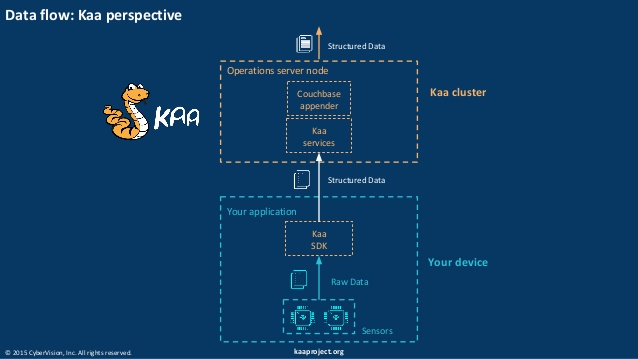
\includegraphics[scale=0.5]{images/kaa_platform1}
\caption{Flujo de datos en Kaa}\label{L502}
\end{figure} 
\subsection*{Esquemas de datos}
Los datos se recolectan desde los endpoints y se envían al servidor en el formato definido por el 'log schema', previamente creado por el desarrollador para la aplicación en concreto. En la figura \ref{L503} se muestra una arquitectura de los datos. Log Schema usa un formato compatible con Apache Avro. El desarrollador define cómo quiere que se envíe y almacenen los datos mediante estos esquemas, lo que hace a la plataforma muy flexible, facilitando la integración entre los diferentes servicios.\\

Entre el servidor y los endpoints se pueden usar diferentes tecnologías o protocolos, como TCP, HTTP, XMPP, CoAP o MQTT. 

\begin{figure}[H]
\centering
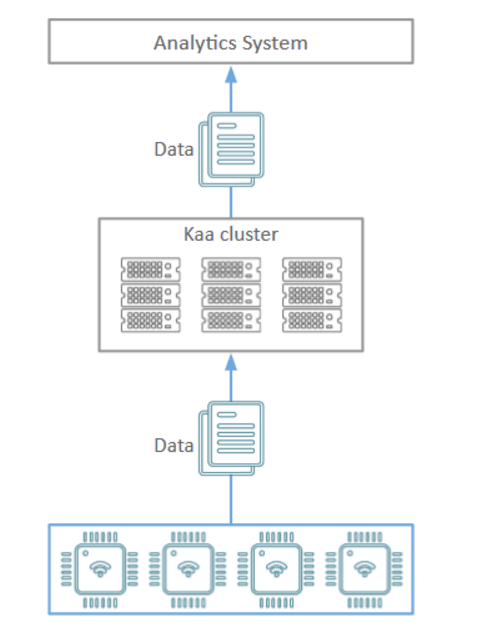
\includegraphics[scale=0.4]{images/log_schema}
\caption{Arquitectura de los esquemas de datos}\label{L503}
\end{figure} 


\begin{figure}[H]
\centering
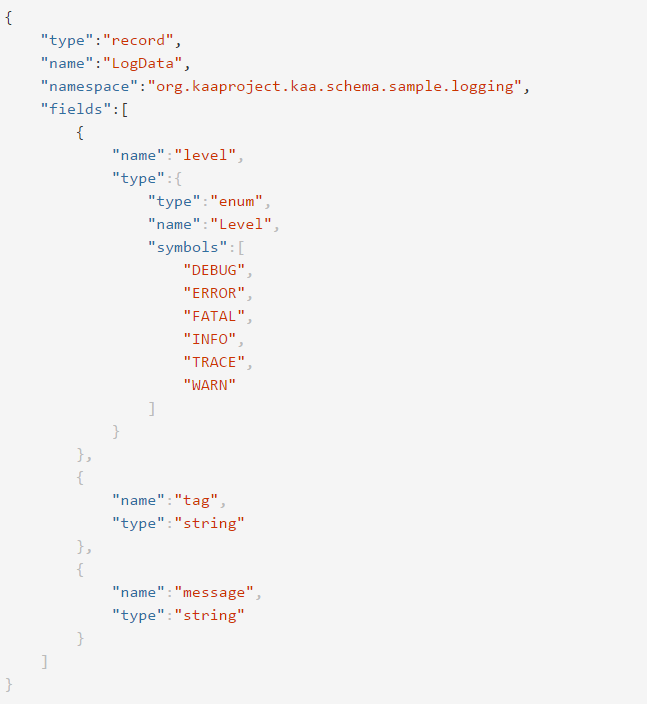
\includegraphics[scale=0.5]{images/log_schema_example}
\caption{Ejemplo de Log Schema}\label{L504}
\end{figure} 
\subsection{Qué ofrece Kaa}
Evaluando a Kaa como middleware IoT, se puede decir que cumple con una gran cantidad de requisitos esenciales. ////////Se va a evaluar como el resto de middleware analizados, es decir, mediante la evaluación de los requisitos presentes en la tabla de la figura \ref{L505} ////////
\begin{figure}[H]
\centering
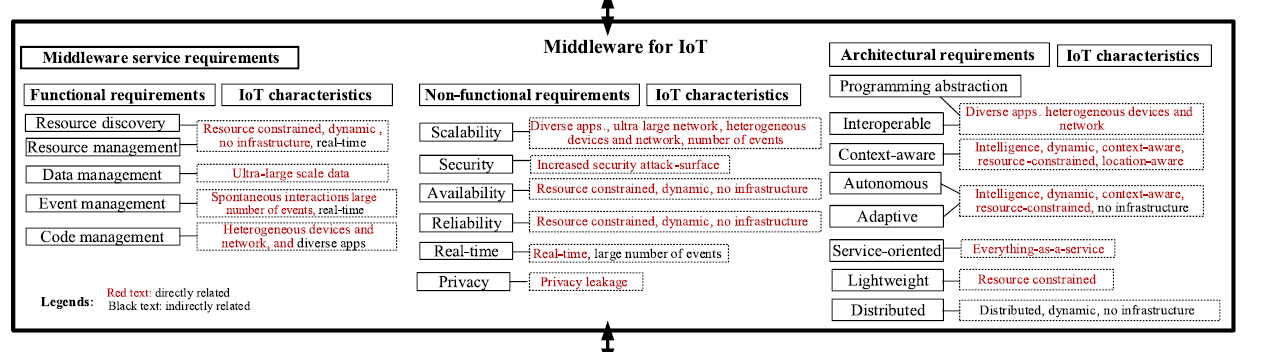
\includegraphics[scale=0.5]{images/requisitos}
\caption{Requisitos de un middleware IoT.}\label{L505}
\end{figure} 

\subsubsection*{Descubrimiento de recursos}
Kaa ofrece un sistema de eventos que permite enviarlos tanto a los diferentes endpoints como al servidor. Al igual que el almacenamiento de datos, los eventos se definen mediante esquemas. La siguiente figura muestra un diagrama de cómo se generan y procesan los eventos. Estos eventos se pueden usar para avisar al resto de endpoints de la aparición de un nuevo recurso (endpoint).
\begin{figure}[H]
\centering
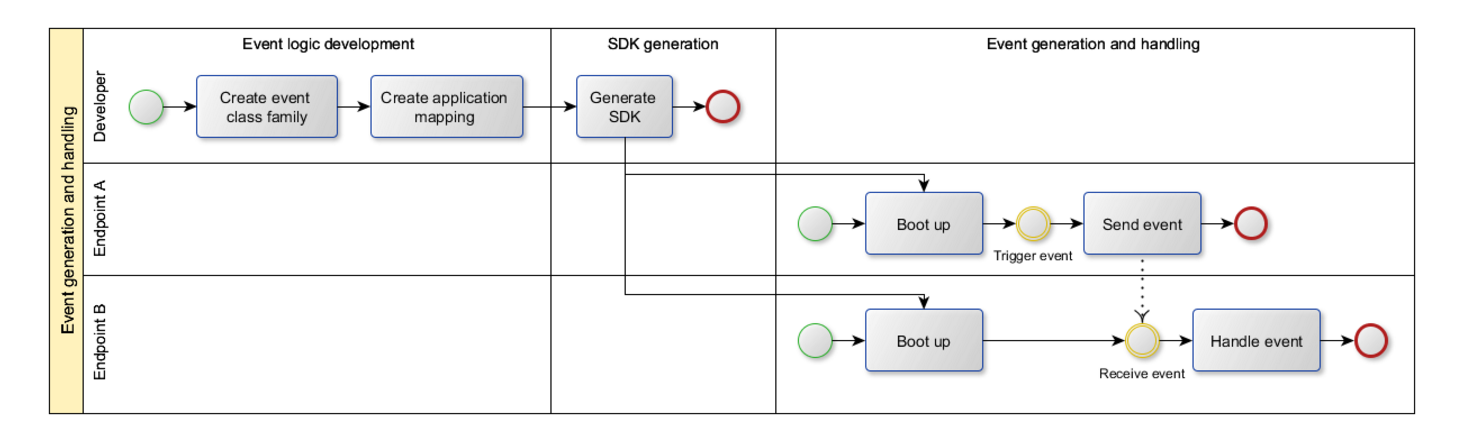
\includegraphics[scale=0.5]{images/events_schema}
\caption{Diagrama de eventos en Kaa}\label{L505}
\end{figure} 

 ///////////////////////////////////////////////////////////////notificaciones basado en tópicos, entregando los mensajes a los endpoints subscritos. Al igual que el almacenamiento de datos, las notificaciones se definen mediante esquemas. Para el envío de mensajes se usan grupos y perfiles endpoints./////////////////////////////////////////////////////////////////////

\subsubsection*{Control de recursos}
En IoT se busca que los recursos puedan ser controlados para que, por ejemplo, se pueda reaccionar ante un fallo de éstos. Kaa no ofrece un control de recursos como tal, pero haciendo uso de los eventos y notificaciones se puede conseguir tal propósito. Por ejemplo, una solución sencilla podria ser que un endpoint guarde cada 5/10 min un valor característico, como su timestamp y, mediante un sistema de análisis, analizar los datos y, en caso de fallo, enviar un evento o notificación a un endpoint en concreto, que será el encargado de reaccionar ante tal efecto. Por ejemplo, avisando a un nodo de monitorización para que intente restablecer el endpoint caído.\\
Otro ejemplo podría ser implementar en un SDK una función 'ping' a la que, haciendo uso del sistema de eventos de kaa, tengan que responder todos los endpoints en un determinado tiempo, si no lo hacen se podría considerar como endpoint caído y actuar ante tal efecto.\\
Por tanto, el sistema de eventos y notificaciones es un sistema muy completo con el que se pueden realizar muchas funciones. Toda funcionalidad tendrá que ser implementada en los endpoints, donde podrán ser conectados a servidores para realizar funciones mas complejas. El motivo por el cual se usa Kaa es, sin duda, su robustez y heterogeneidad con distintas plataformas así como su facilidad de uso. 



...(en un proyecto de kaa en la salud habla de control y configuración de los dispositivos de forma remota. Se podría conseguir mediante eventos???)

\subsubsection*{Control de datos}
Los datos son la principal característica de las aplicaciones IoT, cuando se habla de datos se hace referencia principalmente a los recopilados por los sensores. Un procesamiento, almacenamiento así como una monitorización o filtrado de datos es fundamental para poder desarrollar una aplicación IoT. \\ 

Kaa, a diferencia de otras plataformas comerciales, no ofrece un procesamiento o visualización de datos. En kaa tan solo se almacenan los datos provenientes de sensores. A pesar de que no ofrezca herramientas de análisis de datos como tal, se pueden usar herramientas externas. \\
Con estas herramientas se recopilan los datos almacenados en Kaa de manera que sean estas herramientas las que gestionen los datos. Para comunicarse con los EndPoints se usan las notificaciones Kaa mediante su API.
Más adelante se verá un ejemplo práctico sobre esto, en el que se ha usado Apache Zeppelin como herramienta para el análisis de datos y Cassandra como base de datos de Kaa. Una vez analizados, si supera un cierto umbral, se envía una notificación a Kaa para que encienda un LED en la raspberry.
En la figura ---- se puede ver un esquema de uso con Apache Storm.
\begin{figure}[H]
\centering
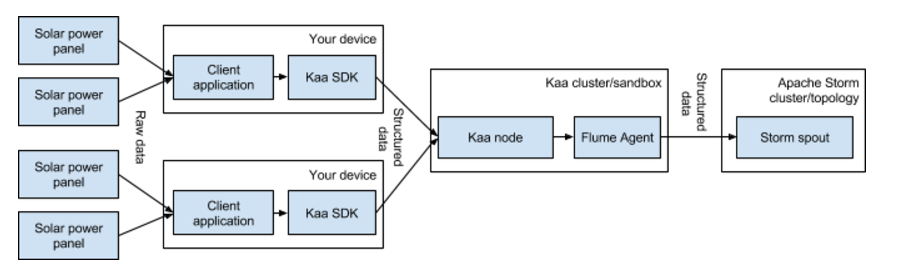
\includegraphics[scale=0.6]{images/esquema_apache}
\caption{Esquema de uso para la monitorización de datos con Apache Storm}\label{L505}
\end{figure} 

\subsubsection*{Escalabilidad}
La plataforma Kaa ha sido diseñada para ser escalable horizontalmente. Se pueden añadir miles de endpoints al mismo nivel, es decir no puede haber varios niveles en la jerarquía. Para poder agrupar distintos endpoints se puede hacer uso de los grupos de endpoints (endpoint group).

\subsubsection*{Tiempo real}
///////////////////Kaa está diseñado para que soporte virtualmente cualquier protocolo de transporte, por ello permite a los desarrolladores usar diferentes protocolos de transporte de datos para diferentes acciones, en el mismo Endpoint. Por defecto se usa HTTP sobre TCP para la comunicación SDK y cluster./////////////////////////\\
Kaa es un sistema en tiempo real, entendiendo tiempo real como unos ms de retraso. Kaa usa HTTP sobre TCP para la comunicación entre SDK y Cluster, por tanto, por definición es un servicio con retardos, aunque despreciables para el escenario que se plantea.


\subsubsection*{Disponibilidad}
Kaa es un sistema con una alta disponibilidad. Está formado por clusters, donde cada cluster representa un servidor. Estos clusters están interconectados mejorando así la disponibilidad en caso de fallo de alguno de ellos. Para la coordinación entre los diferentes nodos Kaa usa Apache Zooekeeper. Además, los datos de los endpoints se almacenan en bases de datos tolerantes a fallos.
\begin{figure}[H]
\centering
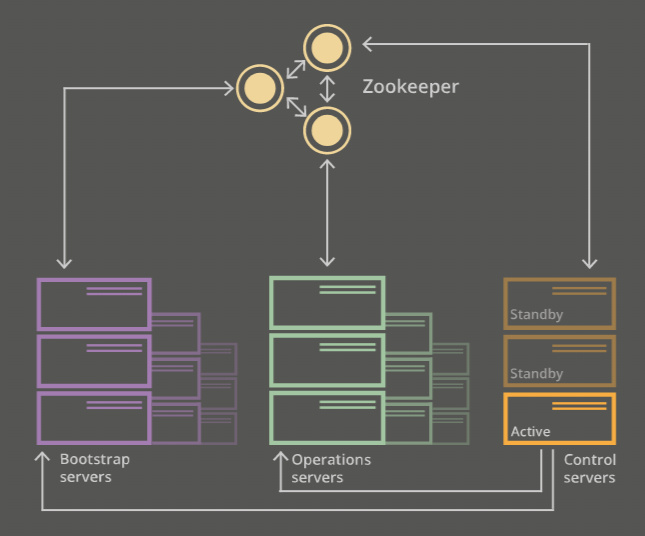
\includegraphics[scale=0.5]{images/disponibilidad_captura}
\caption{Esquema Zooekpeer en Kaa}\label{L506}
\end{figure} 

\subsubsection*{Seguridad y privacidad}
Por defecto, en la comunicación entre Kaa y el SDK se usa una encriptación con RSA y AES. Kaa también asegura un almacenamiento de datos seguro en la base de datos así como la autenticación en la plataforma. Kaa usa el hash SHA-1 de la clave pública como identificador del endpoint en el sistema.
\begin{figure}[H]
\centering
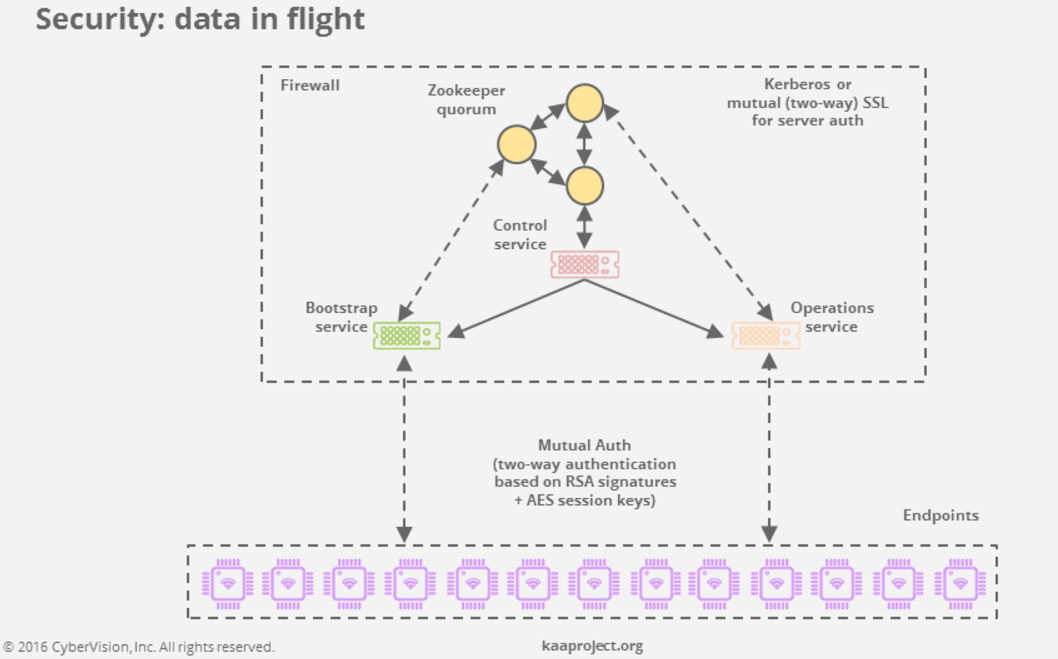
\includegraphics[scale=0.5]{images/security_capture}
\caption{Seguridad en Kaa}\label{L507}
\end{figure} 



\subsubsection*{Popularidad}
Kaa es un middleware reciente y con mucho soporte y documentación, lo que facilita su despliegue.
\subsubsection*{Facilidad para su despliegue} 
Kaa es un middleware que ofrece facilidades para su desarrollo. Dispone de una versión en una maquina virtual ya preconfigurada con aplicaciones y ejemplos de uso de la plataforma. El uso de SDKs facilita la interoperabilidad de diferentes plataformas sin la intervención del usuario. Con Kaa se consigue que el desarrollador se 'olvide' de la parte del servidor. 

\subsubsection*{Interoperabilidad}
La interoperabilidad de distintas plataformas es una de las características de Kaa, en la que una misma aplicación puede ser desarrollada para diferentes plataformas, tan solo descargando el SDK generado por Kaa. Esto hace que sea una plataforma totalmente heterogénea en cuanto a plataformas se refiere. Un endpoint puede ser ejecutado en distintos dispositivos, desde un teléfono móvil a una raspberry o arduino.


\subsubsection*{Distribuido}
Kaa es una plataforma distribuida, que se organiza en clusters donde cada uno de ellos puede ejecutar una determinada funcionalidad que será controlada como un único sistema. Por defecto, Kaa está formada por un único cluster ejecutando el servidor Kaa. 




\subsubsection*{Abstracción de la programación}
Kaa proporciona una interfaz al desarrollador, posibilitando una sencillez a la hora de crear las aplicaciones. El desarrollador tan solo tiene que crear los esquemas de datos, pues la plataforma se encarga de generar el código. Además de la interfaz, Kaa proporciona una API que permite realizar todas las funciones que se pueden llevar a cabo a través de la interfaz, mediante llamadas a la misma. Esto es muy útil a la hora de quien tenga que realizar las funciones sea el endpoint automáticamente, lo que hace que Kaa sea una plataforma autónoma.



\subsubsection*{Basado en servicio}
-----



\subsubsection*{Adaptativo}
Kaa soporta virtualmente cualquier protocolo de red, endpoint o almacenamiento de datos, lo que hace a la plataforma tolerante a cambios.



\subsubsection*{Control de eventos}
-------------



\subsubsection*{Control de código}
Una de las principales características de Kaa es que es Open Source con todo lo que ello implica. El código es totalmente transparente al usuario.


\section{Uso de la plataforma}
\subsection{Instalación}
Para instalar la plataforma hay 2 formas, o bien usar la maquina virtual que ya viene preconfigurada y con unos ejemplos de uso (SandBox)o bien, construir un servidor Kaa propio mediante el código fuente. Todo esto está perfectamente documentado.
\subsection{Partes de la plataforma}
Las características de Kaa son:
\subsubsection*{Eventos}
Kaa proporciona un mecanismo para la entrega de eventos (mensajes) a través de los endpoints. Los eventos pueden ser unicast o multicast, eligiendo así el/los destinatario/s. Los endpoints generan los eventos y los envían al Kaa server, éste se encarga de enviarlos a los endpoints acorde al esquema de eventos, previamente configurado por el desarrollador. La figura \ref{L505} muestra el proceso de envío y recepción de eventos.\\
En el siguiente ejemplo se muestra la definición de un esquema de eventos. El formato está basado en \MYhref{http://avro.apache.org/docs/current/spec.html}{Avro Schema}.
\begin{lstlisting}

{
    "namespace": "com.company.project",
    "type": "record",
    "classType": "event",
    "name": "SimpleEvent2",
    "fields": [
        { "name": "field1", "type": "int"},
        { "name": "field2", "type": "string"}
    ]
}

\end{lstlisting}
Cada evento se basa en una clase en concreto (EC), definida en el esquema de eventos. Una EC se identifica mediante su nombre completo, en el ejemplo de arriba sería: " com.company.project.SimpleEvent2". El identificador es único y no puede haber 2 ECs con el mismo nombre en el mismo tenat ////////////////////////explicar tenat///////////.\\

Por otra parte, las clases de eventos (ECs) se agrupan en familias de clases de eventos (ECFs). Un ECF se identifica por su nombre y/o nombre de clase, por lo que no puede haber 2 ECFs con el mismo nombre o nombre de clase en un mismo tenat. El siguiente esquema muestra un ejemplo de definición de ECF:
\begin{lstlisting}
[
    {
        "namespace": "com.company.project.family1",
        "name": "SimpleEvent1",
        "type": "record",
        "classType": "event",
        "fields": []
    },
    {
        "namespace": "com.company.project.family1",
        "name": "SimpleEvent2",
        "type": "record",
        "classType": "event",
        "fields": [
            { "name": "field1", "type": "int" },
            { "name": "field2", "type": "string" }
        ]
    }
]
\end{lstlisting}
\subsubsection*{Colección de datos}
Los endpoints almacenan datos recopilados ("log") siguiendo una estructura predefinida. El SDK implementa la subida de 'logs' desde los endpoints al servidor. El servidor lo almacena en bases de datos. En el siguiente ejemplo se muestra un simple esquema de almacenamiento de datos (log schemas), compatible con \MYhref{http://avro.apache.org/docs/current/spec.html}{Avro Schema}:
\begin{lstlisting}
{
    "name": "LogData",
    "namespace": "org.kaaproject.sample",
    "type": "record",
    "fields": [
    	{
            "name": "tag",
            "type": "string"
        },
        {
            "name": "message",
            "type": "string"
        }
    ]
}
\end{lstlisting}
La especificación de la base de datos se hace mediante log appenders usando la interfaz de usuario. 
\subsubsection*{Perfiles y grupos}

\subsubsection*{Notificaciones}
Kaa dispone de un sistema de notificaciones para la entrega de mensajes desde el clúster Kaa hasta los endpoints. La estructura de los datos se define en el esquema de notificaciones, configurado en el servidor y desplegado dentro de los endpoints. Las notificaciones a tópicos de forma que para recibir una notificación, el endpoint tiene que subscribirse a uno o varios tópicos. También, se puede asignar un tópico a todo un grupo de enpoints. El envío de notificaciones se puede hacer mediante la interfaz de usuario o mediante una llamada a la API. 
\begin{figure}[H]
\centering
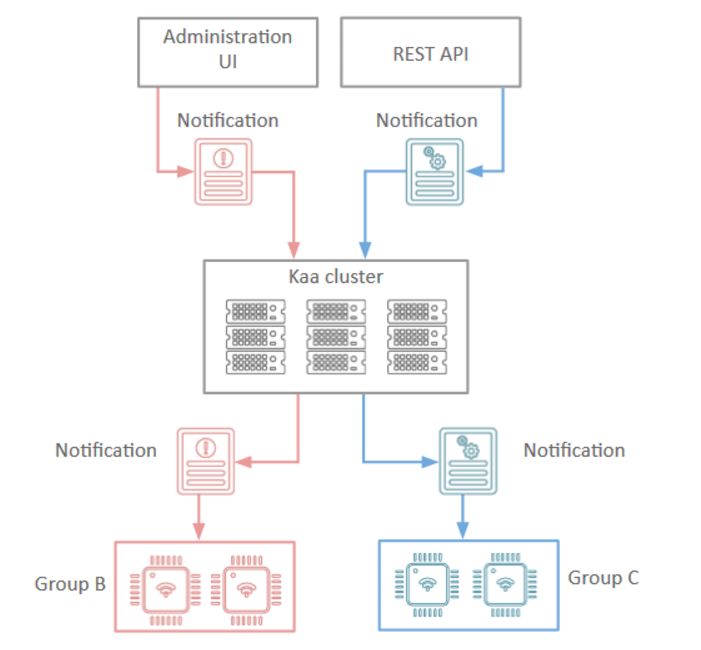
\includegraphics[scale=0.5]{images/notifications}
\caption{Notificaciones en Kaa}\label{L508}
\end{figure}
\subsubsection*{Distribución de datos}
La distribución de datos es una de las principales características de Kaa ya que los desarrolladores pueden definir cualquier tipo de datos mediante los esquemas de Kaa.
\subsubsection*{Abstracción en la capa de transporte}
Kaa ha sido diseñada para soportar virtualmente cualquier protocolo de transporte de datos. Además se pueden usar diferentes protocolos en un mismo endpoint, por ejemplo las notificaciones mediante SMS y la configuración y datos mediante TCP. /////////explicar virtualmente e incluirlo si consigo usar MQTT como protocolo de transporte////////////
\begin{figure}[H]
\centering
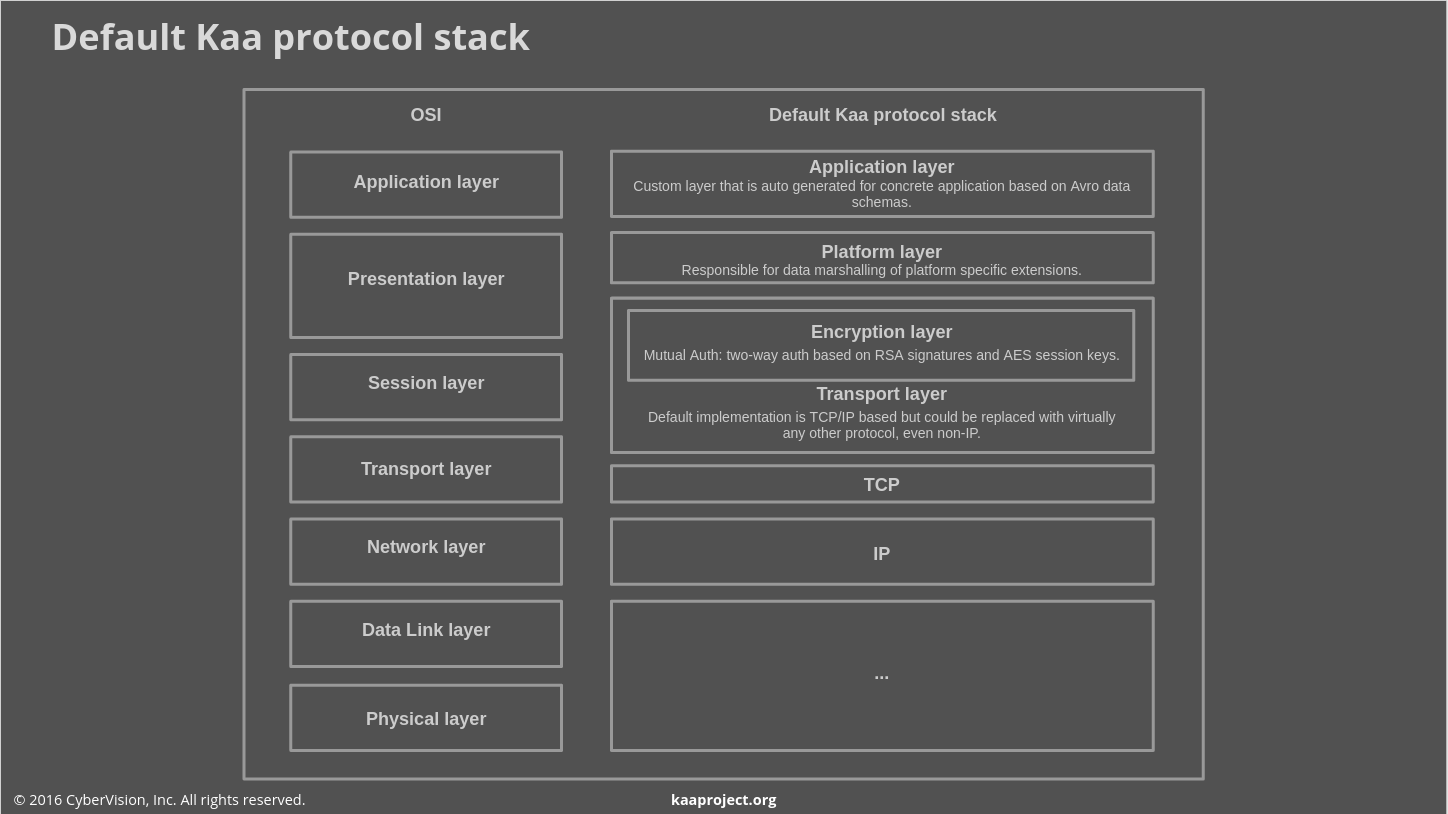
\includegraphics[scale=0.4]{images/kaa_stack}
\caption{Pila de protocolos de Kaa}\label{L508}
\end{figure}
\section{Casos prácticos}

\subsection{Encender un LED en la raspberry usando Kaa}
\subsubsection*{Enviar datos desde la raspberry a Kaa}
\subsubsection*{Analizar datos con Apache Zeppelin}
\subsubsection*{Envío de notificaciones a la Raspberry para encender un LED}

\section{Problemas encontrados}
\end{document}